\documentclass{article}
\usepackage[utf8]{inputenc}
\usepackage[english]{babel}
\usepackage{imakeidx}
\usepackage{listings}
\usepackage{xcolor}
\usepackage{minted}
\usepackage{dashrule}
\usepackage{svg}
\usepackage{pdfpages}
\usepackage{mdframed}
\usepackage{fbox} 
\usepackage{caption}
\usepackage[]{algorithm2e}
\usepackage[T1]{fontenc}
\usepackage{hyperref}

%Color definitions

%---------------------------
\definecolor{joshgreen}{RGB}{78, 154, 6}
\definecolor{bg}{rgb}{0.94,0.97,1.0}
\definecolor{bgshell}{rgb}{0.94,0.9,1.0}
\definecolor{ccol}{RGB}{255,220,220}
\definecolor{commentcol}{RGB}{255, 229, 153}
\definecolor{algo}{RGB}{249,249,239}
\definecolor{servers}{rgb}{0.71, 0.65, 0.26}
\definecolor{properties}{rgb}{0.57, 0.63, 0.81}
\usemintedstyle{perldoc}

%---------------------------


%MD frame styles 

%---------------------------
\mdfdefinestyle{myframe}{%
    linewidth=0.01pt,
    linecolor=grey,
    backgroundcolor=bg,
    nobreak=true
}

\mdfdefinestyle{shell}{%
    linewidth=0.01pt,
    linecolor=grey,
    backgroundcolor=bgshell,
    nobreak=true
}


\mdfdefinestyle{algorithm}{%
    linewidth=0.01pt,
    linecolor=grey,
    backgroundcolor=algo,
    nobreak=true
}

\mdfdefinestyle{hindsight}{%
    linewidth=0.01pt,
    linecolor=grey,
    backgroundcolor=ccol,
    nobreak=true,
    innertopmargin=\baselineskip,
    innerbottommargin=\baselineskip,
    innerrightmargin=20pt,
    innerleftmargin=20pt,
}

\mdfdefinestyle{comment}{%
    linewidth=0.01pt,
    linecolor=grey,
    backgroundcolor=commentcol,
    nobreak=true,
    innertopmargin=\baselineskip,
    innerbottommargin=\baselineskip,
    innerrightmargin=20pt,
    innerleftmargin=20pt,
}

\lstset{keywordstyle=\ttfamily\color{purple},language=C}
\def\inline{\lstinline[basicstyle=\ttfamily,keywordstyle={}]}

\lstset{
    language=C,
    basicstyle=\ttfamily,
    keywordstyle=\color{purple},
    commentstyle=\color{darkgreen}
}

%---------------------------


%Commands
%---------------------------
\newcommand{\hindsight}[1]{
\begin{center}
\vspace{0.5cm}
\begin{minipage}{0.9\textwidth}
\begin{mdframed}[style=hindsight]
\textbf{Hindsight}




\vspace{0.1cm}
\textit{#1}
\end{mdframed}
\end{minipage}
\vspace{0.5cm}
\end{center}
}


\newcommand{\comment}[1]{
\begin{center}
\vspace{0.5cm}
\begin{minipage}{0.9\textwidth}
\begin{mdframed}[style=comment]
\textbf{Comment}




\vspace{0.1cm}
\textit{#1}
\end{mdframed}
\end{minipage}
\vspace{0.5cm}
\end{center}
}

\newcommand{\C}[1]{
\lstinline{#1}%{\fontfamily{qcr}\selectfont #1}
}

\newcommand{\N}[1]{\newline\newline\textit{#1} \hdashrule[0.5ex]{12cm}{0.5pt}{3pt} \newline\newline}

\newcommand{\EN}{\newline\newline\hdashrule[0.5ex]{13cm}{0.5pt}{3pt} \newline\newline}

\newcommand{\josh}[1]
{\ttfamily{\bfseries\color{joshgreen}josh}\color{black}\ \$ #1}

\newcommand{\bash}[1]
{\ttfamily{\bfseries\color{joshgreen}bash}\color{black}\ \$ #1}
% \cline{}

\newenvironment{code}{\captionsetup{type=listing}}{}

\setlength{\parindent}{0em}
\setlength{\parskip}{1ex}
%---------------------------

\if 0

Struktur:
A detailed description of the core of the OS you built as a group:
    - MM %Roman
    - Vspace -> - Page fault handling %Vspace + Pagefault handler
    - Processes, threads, dispatch (only spawning) %Franz
    - Multicore %Multicore
    
    - Message passing %Nico
        -> Overview
        -> LMP
        -> UMP 
    

        



A section containing descriptions of the individual projects you undertook:
    Individual 
    -> File
    -> Shell
    -> Name
    -> Networking

An evaluation of the performance of the OS you have built:


Evaluations: 
-> MM
-> pagefault handle
-> malloc -> 

A user guide for the OS, explaining how to run its functionality and any particularly important programming interfaces:
    -> Basic use
    -> shell usage
    -> core programs that can be used
    -> how to write a program using our interfaces


\fi









\lstset{
    frameround=fttt,
    language=C,
    numbers=left,
    breaklines=true,
    }
    
\lstMakeShortInline[columns=fixed]|


\if 0

\section{Notes}
\subsection{Foreword}
\N{Franz}
How we proceed with tasks: First, we build a simple and mostly straight forward base structure. With that working, we have a solid and hopeful stable base to build upon on and improve our structure. From then on, we have also the option to experiment with new ideas and algorithms. 
\EN
\subsection{Milestone 1 - 18.03.2020}
\N{Franz}
\EN


\subsection{Milestone 2 - 25.03.2020}
\subsubsection{Base structure}
\N{Nico}
As we do not yet have to implement the \C{paging_unmap} function, we opted for a simple approach
for the vspace management.
\EN
\N{Franz}
Vspace mapping as a pointer/address (\C{current_virtual_free_address}) in \C{paging_state}. We increment this address each time we allocate virtual address space. This first solution works only with the current assumption that the vspace will never be fully utilised. 

elf address map to virtual address to read.
\EN

\N{Nico}
We use this vspace management system to implement the next steps of the milestone. It works for our purposes now, as we never exhaust a 48-bit address space. However, we absolutely need to come back to this and implement it so it allows freeing memory as well. If not, we will eventually run out of virtual address space. If we want to design a system that can sustain memory-intensive processes or run for a long time without rebooting, this is a no-go.

With the vspace management working, we moved on to implementing the first part of process creation -- Creating the child's cspace and vspace.

As a next step, we want to load the ELF-file into the child's address space. The elf library in our source tree is designed to help us with that. It provides the function \lstinline{elf_load}, which
needs a callback function that maps some memory to some specific location in the child process, and maps the same memory into the current virtual address space in order to write to it. Implementing this
function seemed rather straight-forward, but as we later discovered, we made a small mistake, that cost us two days of debugging.
\EN



\subsection{Milestone 3 - 31.03.2020}
\N{Franz}
- lmp message from d1 to d2, what happens step for step
prozess wird erstellt mit ep cap from parent
lmp init, aos rpc init (lmp chan init, init bindings, get cap from called), register handlers, send msgs...
waitset expl.: zentrale datenstruktur wo sichmerkt, bei welchem event was aufgerufen werden soll. und dann die richtigen eventhandler called
schribe anenn ort, kernel aufruf, kernel luegt git e reaktion (write or reject, upcall ime andere prozess dass was zum lese verfüägbar isch)

This method works also when the dispatchers are not running on the same core, i.e. they don't share the same CPU Driver.

- explain how a channel is created
1:1 verbindung mit endpoints als "telefonnummer"

- explain in terms of network protocol (Roman), hanshake, 

- demonstration (nico):
    1. invoke an endpoint capability and receive a message on the same cap in other domain (nico)
    2. demostrate rpc implementation, show that it works (code explain: franz + nico / show that messages work well / interface könnte auch für cross-core funktionieren) 
    3. demo spawn new domains upon request (franz)
    4. demo & explain memory server for multiple domains (code explain: nico)
    5. demo & expl termial service (code explain: roman)
    6. extra1: passing large messages (franz)
    7. extra2: terminal read (matt)
    8. extra3: cycle counter (franz+nico)

\EN










% \N{Nico}

% When handling a page fault our page fault handler first does a lookup in which paging region the 
% page fault occurred.

% \begin{itemize}
%     \item In the \emph{vaddr region} and \emph{meta region}, we treat all page faults as
%     fatal errors. This is, as allocations/deallocations in these regions should only ever be done by
%     the aos library i.e. our system code. Trying to access any non-mapped page is certainly an error.
%     \item In the heap region, we proceed differently: On any access to a non-mapped page,
%     we allocate a frame and map it at the fault address. This allows us to let malloc manage the heap and only lazily allocate the necessary RAM to back it up.
%     When first implementing the page fault handler, we always allocated and mapped 4KiB frames.
%     However this proved to require the creation of a lot of capabilities. We therefore changed the size of the allocated frames to 2MiB. Also see \textbf{TODO}
%     \item The stack regions are handled similarly to the heap region. However in the stack regions, we pre-map one page at the beginning of the region that is neither readable nor writable. If we pagefault on this pre-mapped page, we print that a (non-recoverable) stack overflow occurred.
    
%     This works, because the stacks in our system grow from high addresses to lower ones. As a stack starts growing at the end of its paging region, we lazily allocate pages until we are at the start of the region where we will (in most cases) fail with an understandable error message. In the stack,
%     we kept the fine-grained 4KiB chunk size for lazy allocation since stacks are generally of a smaller size than data structures in the heap. % THIS IS NOT TRUE ANYMORE --> rewrite this and hint to this 
    
    
%     \begin{mdframed}
%     \paragraph{Comments}
%     One might question why we map a non-readable non-writable page at the start of every stack region. When handling a page fault within the stack region, the pagefault handler can easily check at which position in the stack region the access occurred and fail with a stack overflow exception without having mapped a page in it.
%     \end{mdframed}
    
% \end{itemize}

% \EN{}

% The user-level address space storage format; what data structures do you maintain, and why?
% Vaddr -> linked list and shadowpagetable


% The fields in the \C{struct paging_state}, and how are they used?

% \EN

\EN{franz nico}
    mega vill schneller wenn mm 2mb pages zrugg git
    assert statements im cap delete: vo wennt childs machsch bi mmalloc, denne löschisch de parent cap und das isch z.t. 20ms ime syscall
\EN


\subsection{Milestone 5 - 29.04.2020}

\subsubsection{frame sharing barriers}
\N{roman}

\subsection{Milestone 6 - 6.05.2020 }
\subsection{Milestone 7 - 3.06.2020 }


% \section{MM}
\N{Roman}
Possible speedup for MM
\begin{itemize}
\item keep 2 linked lists
\begin{itemize}
\item 1 for all nodes
\item 1 for free nodes
\item add according prev / next references to struct mmnode
\end{itemize}
\end{itemize}
\EN

\fi




\begin{document}

\begin{titlepage}
\Huge
\title{\textbf{AOS Report}}
\author{Roman Niggli, Nicolas Winkler, Franz Knobel, Matthew Weingarten}
%\date{March 2021}
\maketitle

\vspace{3cm}
\begin{center}
    \Large
    Advanced Operating System\\
    ETH Zürich\\
    \date{}
\end{center}
\end{titlepage}
\newpage

\makeindex
\tableofcontents


\newpage
\begin{abstract}
 \emph{   A RAM cap, a Frame cap and a NULL cap walk into a bar. The bouncer asks them to identify themselves. Immediately the bar crashes and shuts down.}
\end{abstract}
\newpage


\section{Prelude}

In this course, we completed several assignments, each being part of one big project.
Starting from an initial handout, step by step, we implemented several core parts of an operating system.

Already after a few weeks, we noticed the importance of clean and simple interfaces,
good communication, and improved our skills in understanding pre-existing code.

Over the course of this semester we gained a lot of new perspectives on the design of Operating Systems.
With mostly superficial knowledge about common Operating Systems, we had several moments
of realization that things we assumed inherent to an OS don't need to be. The further
the project went on, the more we understood the often-heard answer ``That is a design
decision which is up to you'' -- There is really no correct way, just multiple ways, each
with its pros and cons.

Looking back on our finished\footnote{at least more or less} project, we almost have a 
hard time accepting that course is already over. We now see so much more
that could be improved or implemented in our system. However realistically speaking,
we can say that we are quite happy and proud of our work.

\if 0

mir hennd de kurs gnah, will eus dgrundlage und dkonzept vo operating systems fasiziniert und interessiert. um das wüsse zvertüüfe hennd mir praktischi erfahrig welle sammli und dhoffnig gha konzept ala learning by doing besser zverstah.
d milestones hennd eus usegfordered und di einzelne baustei vome basic operating system zeiget. 
mir hend gseh und glernt wie die baustei voenand abhängig sind und ufenand ufbaued.
so hennd mir am schluss es funktionierends sehr sehr basics betriebsystem zemebastled. 
es mag nöd s beschte si. heck, nödma guet, aber es söll euses glernte wüsse zu de basics zu operatingsystems und was mir glernt hend idere zit widerspiegle

Wie wichtig d teamarbet und dokumentation vo code isch het sich idem projekt starch bemerkbar gmacht. mit underschidliche codestyles bruchts e codesyle guide und gueti absprache. mir hend glück gha es sones guets team zha. mr seit ja, ds team isch so starch wi sis schwächschte glied und jedi schwächene vo eus sind vo stärchene vo anderne usgliche worde. 

by examining common issues through the lens of barrelfish we gained a new ... profound... complexity operating systems

the eyebrows must be mentioned... 
\fi

\section{Memory Manager}
When booting up, we receive a number of address regions of physical memory from multiboot.
These chunks will be the RAM that our system works with. For our first real milestone,
we implemented a module that manages the distribution of this RAM. Each part of our system,
when needing some memory, will one way or another have to go through this module.

Our memory manager needs to support two main functions: It needs to be able to allocate memory in the form of RAM capabilities, and it needs to be able to free allocated RAM after it is no longer used. Our memory manager is capable of splitting available memory regions, depending on how little memory is required. Lastly, to avoid steady fragmentation, our memory manager will also try and possibly merge memory regions once they have been freed again. See listing \ref{code:mm_state} for an overview of the memory manager's state information.




Perhaps the most important element of an \C{mm} instance is its \C{head}, for without a head a body is but a mindless corpse. A memory manager's \C{head} is a pointer to the lowest address node it manages. Furthermore, every \C{mmnode} has the two members \C{next} and \C{prev}. Through these two pointers, the \C{mmnode} instances managed by our manager form a doubly-linked list. During its initialization, this linked list gets populated with all nodes to manage, ordered according to their base address. A crucial invariant of our memory manager is that this list \emph{always is ordered according to the node's addresses.}

Since our memory manager should be able to quickly find and manipulate available nodes when required, it also has the members \C{free\_head} and \C{free\_last}, pointing to the second list of \C{mmnode} instances. This list is linked through the members \C{free\_next} and \C{free\_prev} in the \C{mmnode} struct, and it only contains free nodes. Without this additional linked list, allocating memory required looping through the first list of nodes, in memory order, until a free node of sufficient size was found. Not only did this waste time by iterating over-allocated nodes, but it also concentrated most activity to a small region of memory, wasting further time through constant fragmentation and defragmentation when other nodes still were available.
\begin{code}
\begin{mdframed}[style=myframe]


\begin{minted}[xleftmargin=\parindent,linenos,breaklines]{C}

struct mmnode {
    enum nodetype type;       ///< Type of `this` node.
    struct capinfo cap;       ///< Cap in which this region exists
    struct mmnode *prev;      ///< Previous node in the list.
    struct mmnode *next;      ///< Next node in the list.
    struct mmnode *free_next; ///< next node in the free-list
    struct mmnode *free_prev; ///< previous node in the free-list
    genpaddr_t base;          ///< Base address of this region
    gensize_t size;           ///< Size of this free region in cap
};

struct mm {
    struct slab_allocator slabs;  ///< Slab allocator used for allocating nodes
    slot_alloc_t slot_alloc_priv; ///< Slot allocator for allocating cspace
    slot_refill_t slot_refill;    ///< Slot allocator refill function
    void *slot_alloc_inst;        ///< Opaque instance pointer for slot allocator
    enum objtype objtype;         ///< Type of capabilities stored
    struct mmnode *head;          ///< Head of doubly-linked list of nodes in order
    struct mmnode *free_head;     ///< Head of unordered doubly-linked list of free nodes
    struct mmnode *free_last;     ///< Last of unordered doubly-linked list of free nodes

    /* statistics */
    gensize_t stats_bytes_max;
    gensize_t stats_bytes_available;

    bool initialized_slot;
    bool refilling;

    struct thread_mutex mutex;
};
\end{minted}
\end{mdframed}
\caption{Our Memory Manager's State Information.}
\label{code:mm_state}
\end{code}
With a separate list just for free nodes, the memory manager can simply loop through it until a sufficiently large node is found, and then use it to allocate the requested amount of memory. Furthermore, since this free list is not ordered in any particular way, using it to allocate memory also spreads out the activity more evenly over all available memory. The only cost incurred through this modification is the additional time spent on ensuring the free list's integrity after allocating or freeing memory. Fortunately, however, this can always be done in constant time.

\subsection{The MM-Invariant}
While mentioned briefly before, the core invariant of our memory manager warrants a more detailed description. In essence, the linked list under \C{mm}'s \C{head} and linked with \C{mmnode}'s members \C{free} and \C{prev} is always ordered according to the nodes' base address and size. A more formal description is as follows:
\[
\forall n \in head.\ \big( n.next = NULL \lor
n.base + n.size = (n.next).base \big)
\]

This invariant is crucial because it allows us to merge newly freed \C{mmnodes} very quickly, as it suffices to check only the two adjacent nodes' type. If the node \C{prev} is free as well, it can simply be merged with the current one. Afterwards, the same process can be repeated with the node \C{next} and we are done. This process does not need to loop, as any adjacent free nodes have already been merged with their free neighbors upon being freed themselves.

After merging two nodes, the only thing left to do is to reestablish the integrity of all linked lists, but since both lists are doubly linked, this is straight forward as well. We can keep one of the nodes and adjust its base or size, and discard the other. In doing so, we simply adjust any references pointing to the node to delete so that it is simply skipped in both lists. For a concrete example, see listing \ref{mm:coalesce} for our function to coalesce a \C{mmnode} with its \C{next}. If both are free, the provided node increases by \C{next}'s size and \C{next} is removed from the ordered linked list. Finally, \C{next} is removed from the list of free nodes too.

\begin{code}
\begin{mdframed}[style=myframe]
\begin{minted}[xleftmargin=\parindent,linenos,breaklines]{C}
static bool coalesce(struct mm *mm, struct mmnode *node)
{
    assert(mm != NULL);

    if (node == NULL || node->next == NULL || !capcmp(node->next->cap.cap, node->cap.cap)) {
        return false;
    }

    struct mmnode *right = node->next;

    if (node->type == NodeType_Free && right->type == NodeType_Free) {
        assert(node->base + node->size == right->base);

        node->size += right->size;
        node->next = right->next;

        if (node->next != NULL) {
            node->next->prev = node;
        }

        remove_node_from_free_list(mm, right); // right node no longer usable
        slab_free(&mm->slabs, right);

        return true;
    }
    return false;
}
\end{minted}
\end{mdframed}
\caption{Merging two Nodes and Updating all Linked Lists.}
\end{code}
\label{mm:coalesce}

Complementary to merging nodes, we also have to preserve our invariant when splitting nodes. To do so, all we have to do is create a new node next to the one being split. The new node is then added to the ordered linked list next to the node being split. If the new node also is a free node, we can insert it to the free list as well. But since the free list is not ordered, we do not have to worry about the location at which it is inserted.

%\subsection{Thread Safety}
%Initially, our memory manager did not have to worry much about thread safety. But as our system grew in complexity, we started observing a somewhat rare yet annoying bug. When spawning multiple processes, they request large amounts of memory at the same time. This could in some cases lead to the memory manager retyping the same capability twice. Naturally, such an event caused catastrophic failures whenever it happened, so the logical solution was to add a mutex to the memory manager. Whenever a process requests memory, it has to wait until the \C{mm-mutex} becomes free. Then it locks the memory manager and obtains its memory before finally freeing the memory manager's mutex again.
%
\subsection{Allocating and Freeing Memory}
Based on the above explanation, we now examine how the memory manager provides its core functionality. Namely, how the memory manager can allocate and free memory, how it tracks its available space and how it prevents fragmentation.

To allocate memory of a requested size, the manager simply loops through all its available free nodes. If it cannot find one of at least the requested size, it reports an error. Next, if the found node is located at an unfortunate offset, the memory manager simply splits it to obtain a new node with valid offset. Afterwards, the node's capability is retyped according to the request's type and size before in a last step, our memory manager checks if the node it allocated is larger than the requested size. In case the allocated node is indeed bigger than requested, the remaining part is split into a new free node, as to not waste memory unnecessarily.

Luckily, freeing allocated memory is much easier than allocating it: In a first step, the memory manager has to find the \C{mmnode} corresponding to the capability it is to free. Next, it sets the node's type to free and destroys the provided capability. To avoid fragmentation, the memory manager then tries to merge the freed node with both of its neighbors, before finally adding it to the list of free nodes.

\subsection{The Memory Server}
To make finally make our memory server available to other processes, we decided to keep
it as a part of the init process. However, in order for it to work more independently
from init, we moved all the functionality of allocating memory for different dispatchers
than init into a separate thread.

The memory server implements the backend for a selection of methods in \C{usr/init/mem\_alloc.c}, and we can access them from any dispatcher through corresponding RPC calls (\emph{see Section \ref{message_passing}}). We initialize our memory manager in our init process and start a new thread that constantly dispatches events on its own \C{waitset}. We then provide each process we start up with a direct channel to the memory server so that all of them can request memory independently. The method \C{get\_mm\_rpc} in \C{lib/aos/domain.c} can be used by those processes to obtain this connection and request memory as needed.

Finally, each process that is initialized has to be instructed which function to use when requesting memory. This can be done with the function \C{errval_t ram_alloc_set(ram_alloc_func_t local_allocator)} and every process outside of \C{init} and our memory server has this set to one that simply calls our memory server with an RPC (\emph{see Listing \ref{mm:remote_alloc_fun}}).

\begin{code}
\begin{mdframed}[style=myframe]
\begin{minted}[xleftmargin=\parindent,linenos,breaklines]{C}
void handle_request_ram(struct aos_rpc *r, uintptr_t size, uintptr_t alignment, struct capref *cap, uintptr_t *ret_size) {
    errval_t err = ram_alloc_aligned(cap, size, alignment);
    if (err_is_fail(err)) {
        DEBUG_ERR(err, "Error in remote ram allocation!\n");
    }
}
\end{minted}
\end{mdframed}
\caption{Default RAM Allocator Function: Small Wrapper around an RPC Call.}
\end{code}
\label{mm:remote_alloc_fun}



Since \C{init} is started before our memory server thread, we allow it to allocate memory by
directly calling the functions in the MM module. After the memory server thread is started,
we therefore need to pay attention to race conditions when init and a different dispatcher
request memory at the same time. We solve this problem by simply locking the MM
module for each call. 

%it also has its own RAM allocator function. Finally, for the memory server itself we set the RAM allocator function to be our memory manager's allocator function since the memory server is designed to have exclusive direct access to our memory manager.
\section{Paging}\label{paging}

In this section, we describe how we organized our virtual address space, implemented our paging state, and handle page faults. The memory manager, together with the bookkeeping functionality of the paging infrastructure, handles all memory related operations.


    \begin{figure}[hbt!]
        \centering
        % 
        \scalebox{0.6}{
            \includesvg{./paging/data/virtual_address_layout.svg}
        }

        \caption{Virtual address space layout}
        \label{fig:virtual_address_layout}
    \end{figure}



\subsection{Virtual address layout}
On a high level, the virtual address space is divided into \textit{paging regions}, see listing \ref{code:paging_region}. A paging region is a (mostly large) contiguous block of addresses. The \C{struct paging_region} holds information on the memory subsection defined by this paging region, what the region is used for and how page-faults in this region will be handled. No two paging regions overlap and every address can uniquely be resolved to
belong to a certain paging region. To uphold this invariant, we create one large paging region covering the whole address space at the start, mark that region as free space, and then offer a function to allocate new paging regions, which, similarly to the memory management system, subdivides free regions.

\paragraph{}
At system startup, the first region we split off is the \textit{Global Region}, ranging from address \C{0x0} to \C{VADDR_OFFSET}. This region holds all globally defined data in the Vspace, such as binaries. We treat this region as a black box, where the process that spawned our current process (or the CPU driver in the case of init) allocated data necessary
for spawning.
\begin{code}
\begin{mdframed}[style=myframe]
\begin{minted}[xleftmargin=\parindent,linenos,breaklines]{C}
struct paging_region {
    lvaddr_t base_addr;
    lvaddr_t current_addr;
    size_t region_size;
    char region_name[32]; 
    enum paging_region_type type;
    bool lazily_mapped;
    bool map_large_pages;
    paging_flags_t flags;
    struct paging_region *next;
    struct paging_region *prev;
};
\end{minted}
\end{mdframed}


\caption{Paging regions, dividing and recording the virtual address space }
\newline
\label{code:paging_region}
\end{code}
\paragraph{}



Since, in our system, no information about the layout and mappings
of this region is transferred to the child process, we just accept this region “as is” and never allocate something in it. 
\paragraph{}
The next region, referred to as the \textit{meta region}, is where we map memory used to manage all of the virtual memory system itself and further allocations that take place before malloc is initialized. For example, the data structure keeping track of the memory regions itself is allocated mostly inside this region. This region also holds our shadow page table, described in section \ref{paging_state}. We assigned a size of 8 TB to this region since the shadow page table can potentially get quite large, with a maximum of $512^3$ page table entries, each having $512$ entries, resulting in up to $2^{36}$ entries. Thus, 8 TB or $2^{43}$ b gives us more than enough space to hold a fully loaded shadow page table, including paging and any further allocations made that cannot use malloc.
\paragraph{}
We then define one additional big region as the \textit{heap region}. This is the memory region
passed via morecore to malloc. In our implementation, we set the region to a
fixed size of 4TB, this should be enough for all current purposes of our system. Further regions are added dynamically on demand. In most cases, these are Stack regions containing the stacks of newly spawned threads. There are multiple reasons for this splitting of the virtual memory space. It simplifies memory management, as there are different strategies applied to different
regions. Most importantly however is that we handle page faults differently
depending on which region they occur in. Figure \ref{fig:virtual_address_layout} shows the full picture of our virtual address space division into regions.

\subsection{Paging state} \label{paging_state}


Our paging state stores all the information regarding the paging regions of our virtual address space, and the state needed to map frames, and the current layout of our Vspace. This means the paging state stores a pointer to the shadow page table, a pointer to the special regions for faster lookup, including the threads stack region, and pointer to a linked list containing all regions.

\begin{code}
\begin{mdframed}[style=myframe]
\begin{minted}[xleftmargin=\parindent,linenos,breaklines]{C}
struct paging_state
{
    struct thread_mutex mutex;
    struct slot_allocator *slot_alloc;      
    struct mapping_table map_l0;            
    struct slab_allocator mappings_alloc;   
    bool mappings_alloc_is_refilling;       
    struct paging_region *head;            
    struct paging_region vaddr_offset_region;  
    struct paging_region free_region;   
    struct paging_region heap_region;   
    struct paging_region meta_region;   
    struct paging_region stack_region;  
};

\end{minted}
\end{mdframed}
\caption{Paging state structure}
\newline
\label{code:paging_state }
\end{code}




Now that we understand the overview of our Vspace layout and the paging state, we must provide the utility to map physical addresses, in the form of RAM capabilities, into our virtual address space. To be precise, a RAM capability is an untyped capability, and any memory used in userspace for reading and writing must be retyped to a \textit{Frame} capability. In our case, the responsibility of mapping a Frame into the virtual address space falls on to our paging implementation in userspace. To create a new mapping between a virtual address and a physical Frame capability we must invoke the \C{vnode_map} function. 
\begin{mdframed}[style=myframe]
\begin{minted}[xleftmargin=\parindent,linenos,breaklines]{C}
errval_t vnode_map(struct capref dest, struct capref src, capaddr_t slot,
 uint64_t attr, uint64_t off, uint64_t pte_count,
 struct capref mapping)
\end{minted}
\end{mdframed}

\paragraph{}
However, \C{vnode_map} merely creates an entry in the page table. We must ensure that this function is invoked correctly and we must keep track of the resulting capabilities. Furthermore, we need to keep track of the state of the paging table, which is not necessarily directly exposed to us. To perform this task we created a shadow page table, mirroring the page table entries written onto the \C{ObjType_VNode_AARCH64} capabilities. These read-only frames are used by the MMU for virtual to physical address translation. Our shadow page implementation is shown best by the struct in figure \ref{code:shadow_page_table}. Each instance of \C{struct mapping_table} has a one-to-one relationship with a VNode, and a reference to said VNode stored in \C{struct capref pt_cap}. Each mapping table entry holds a resulting mapping capability of the \C{vnode_map} in the \C{mapping_cap} array. If the instance of a mapping table entry corresponds to an L3 VNode, the children pointer array stays empty, as these Nodes correspond to the leaf of the paging tree.

\begin{code}
\begin{mdframed}[style=myframe]
\begin{minted}[xleftmargin=\parindent,linenos,breaklines]{C}
struct mapping_table
{
    struct capref pt_cap;

    struct paging_region *region;

    struct capref mapping_caps[PTABLE_ENTRIES];

    struct mapping_table *children[PTABLE_ENTRIES];
};
\end{minted}
\end{mdframed}
\caption{Shadow page table structure}
\newline
\label{code:shadow_page_table}
\end{code}





\comment{
Currently in our system the mapping capabilities are never actually used. However, if we wished to extend our implementation, for example to support the unmapping operation, this would require us to have access and the ability to invoke these capabilities. I.e the mapping capabilities serve as our access rights to update the paging table.
}




\paragraph{}
Following this logic, our main function for handling the mappings is
\begin{mdframed}[style=myframe]
\begin{minted}[xleftmargin=\parindent,linenos,breaklines]{C}
paging_map_fixed_attr(struct paging_state *st, lvaddr_t vaddr,struct capref frame, size_t bytes,int flags
\end{minted}
\end{mdframed}
the pseudocode is shown in algorithm \ref{alg:paging_map_frame}. The idea is, given a virtual address, a frame capability and the size of the physical frame to: (1) create an entry in the page table used by the MMU for the translation, and (2) keep track of this mapping in our shadow page table, only used by our process in user-space for bookkeeping and further mapping operations.


\begin{mdframed}[style=algorithm]
\begin{algorithm}[H]
\SetKwInOut{Input}{input}
\Input{vaddr, frame, size}

  \emph{chunks} $\leftarrow $  split frame into chunks of size \C{BASE_PAGE_SIZE} \\
  \emph{page table entry }$\leftarrow $ \C{ROOT_PAGE_TABLE}\\
 \For{chunk in chunks}{
    \For{$i\leftarrow 3$ \KwTo $1$ }{
        \emph{pt\_index} $\leftarrow $ \emph{vaddr$[(12 + i * 9) :: (12 + (i - 1) * 9)]$} \\
        \emph{page table entry}$\leftarrow $ \emph{page table entry}$[pt\_index]$ \\
        \eIf{page table entry \textbf{is} NULL}{
            \tcc{Table entry of level i has to be created} \\ 
            
            Create new \C{struct mapping_table} \;
            Allocate a VNode capability\;
            Map VNode with \C{vnode_map} \; \\ 
            
        }
    }
    \tcc{Reached a Leaf Page table entry}\\ 
    \C{vnode_map(pt table entry,chunk,pt_index} \\
    Store resulting mapping in \C{mapping_caps}$[pt\_index]$\\ 
 }
 \caption{The function to map frames into VSpace using our shadow page table}
 \label{alg:paging_map_frame}
\end{algorithm}
\end{mdframed}

\paragraph{}
The index into the page table entry is described by a subset of 9 bits in the virtual address of the desired mapping. The 12 LSB are discarded for the translation, as they are translated one-to-one. This is because the smallest possible unit of mapping is 4KiB, i.e the \C{BASE_PAGE_SIZE}. The following sets of 9 LSB are used to index into the different levels of the page table, mirrored in our shadow page table.
\paragraph{}
Using these indices we can walk the page table. Whenever a page table index has a \C{NULL} entry in our shadow page table, we can infer that the page table for virtual address translation also does not have the corresponding page table entry. Therefore, whenever we encounter a reference to \C{NULL}, we must allocate a new VNode with the correct type, consistent with the level of the page table entry. Furthermore, this VNode must also be mapped into the page table entry and shadow page table and is written to be mapped into the VNode one level higher in the hierarchy. This is one of the reasons which motivates the implementation of a shadow page table, such that we can always keep track of exactly which VNodes have yet to be mapped.

\paragraph{}
Once the leaf node instance of the shadow table has been reached, we have all the information required to invoke the kernel, create a new entry in the page table and receive a mapping capability, completing the operation.

\paragraph{Large Pages}
It is also supported on aarch64 to directly map frames of either 2MiB or 1GiB directly into
either a level 2 or level 1 page table\footnote{There are even more supported
page sizes, however changing that would require a bit more changes to the system}.
In our system, we implemented support for mapping frames directly in the L2 page table.
For this, a frame needs to be aligned to 2MiB (its physical address), and also the virtual
address we want to map it at needs to fullfill this alignment. See Section \ref{sec:slow_mem}



\subsubsection{Locking the paging state}

Operations on the paging state can happen concurrently over multiple threads and are inherently critical. Bad inter-leavings of threads can result in errors, leaving our mapping table with an inconsistent state, or potentially even worse, assigning a \C{struct region} to two different threads. To prevent this type of behavior and make the paging operations thread-safe, we store a \C{thread_mutex} on the paging state. Any critical operation will first attempt to take the lock before continuing, ensuring any updates to the paging state are seen atomically by other threads.











\subsection{Handling page faults} \label{page_fault_handling}

A page fault occurs when the kernel triggers an upcall into our process in \C{disp_pagefault}. It passes the \textit{address} causing the pagefault, an \textit{instruction pointer} and processor specific \textit{error code}. This upcall disables the previously running thread. Next, the dispatcher forwards the exception to the currently running thread with \C{thread_deliver_exception_disabled}. To explain how we respond appropriately to the page fault we distinguish the different types of pagefaults based on the faulting address:

\begin{itemize}
\item Inside the heap region
\item Inside a stack region
\item Any other address, including  
    \begin{itemize}
        \item Inside the meta region
        \item Outside our virtual address space (\C{>0x0000FFFFFFFFFFFFULL)}
        \item Below the Virtual address offset, inside the global region
    \end{itemize}
\end{itemize}

Of all the region types we have divided our virtual address space into, \textit{only} addresses inside the stack and heap region can be validly resolved by the pagefault handler without throwing an exception and aborting the thread. Both the stack and heap regions are \textit{lazily} mapped and thus allow for on demand paging. 
\paragraph{}
When a pagefault is thrown with an address inside the heap region, this means an access was made to a virtual address inside the heap that has not yet been backed by a physical frame. To resolve the fault we simply allocate a new frame capability, requesting more memory from the memory manager and map it into our virtual address space. Thereafter we exit the pagefault handler thread and resume the previously running thread. Similarly, the stack region may also be paged in on demand. However, to ensure that a stack overflow does not corrupt memory, we check whether the address is the last page left in the stack region. If this is the case, we also throw an exception and abort the thread. To support this on demand paging for stacks, whenever a new thread is created we split  a region from an available free region and assign the addresses thereof to the thread stack pointers.

\paragraph{}
Even further, depending on the region type, we choose different granule sizes for the frame we allocate:
\begin{itemize}
    \item In a stack region, we always allocate frames of size \C{BASE_PAGE_SIZE} (4096)
    \item In the heap region, we generally use a larger amount of memory. Using a small
    page size granularity leads to high ``capability overhead'' in our system. We therefore opted to
    always allocate and map frames of size \C{LARGE_PAGE_SIZE} (2MiB).
\end{itemize}

\comment{ We can't catch all stack overflow errors with certainty, as allocating
huge data structures on the stack might cause us to ``overstep'' the guard region entirely. However these cases are extremely rare, so that they don't legitimize
making the guard region even larger.}

\subsection{Slow Memory System}
\label{sec:slow_mem}

After our initial implementation of the paging infrastructure, we noticed that our paging system was very slow. To test whether our implementation worked
correctly, we wanted to malloc 100 MiB of memory, write to it and read it again. To our satisfaction, everything worked correctly
however the whole process took about 10 minutes.

After investigating the cause of this, we found that a call to \C{frame_alloc} got slower and slower the more it was called.
\C{Frame_alloc} is used in our page fault handler to page in physical frames on demand each time we needed a new one. It requests a ram capability from the memory server,
retypes it to a frame capability and deletes the original ram cap.
Further investigation showed us that it was the deletion that caused almost all of the
slowdown. After allocating sufficiently many frames, we managed to bring the time
needed for one capability deletion i.e. a call to \C{cap_delete}, a single syscall,
taking over 20 milliseconds.

We \textit{feverishly} sought for a spectacular bug that was responsible for this havoc.

What we discovered was something different.
The CPU Driver keeps a large tree-like datastructure containing all capabilities. It always upholds certain invariants for this tree. Several functions operating on this tree have assertions and macros
that check that these invariants are upheld at all times. Some of these assertions require  a whole DFS on the tree for to validate the assertion. As we were always running our code with
assertions enabled, we always performed these checks.
A deletion operation performed therefore several DFSes over the whole capability tree
of the CPU Driver, which explains the more or less linear growth in runtime we observed
for this function.

The effect that disabling assertions has on the speed of allocating memory
can be seen in Table \ref{table:large_paging}. For this example, we
used malloc to allocate 100 MiB of data and then write to every byte.
We measured the time this took both with assertions enabled and disabled,
as well as when the lazy allocation backing up the heap region operates with
4KiB granularity and with 2MiB granularity.
\begin{table}[h]
\begin{center}
\begin{tabular}{c c c} 
     &  2 MiB & 4 KiB \\ \hline 
Assertions enabled & 452\,ms  & 8\,min 44\,s \\\hline  
Assertions disabled  & 384\,ms & 6933\,ms \\  
\hline

\end{tabular}
\end{center}
\caption{Difference of paging speed when using larger page granularity, in debug and no debug mode}
\label{table:large_paging}
\end{table}
\paragraph{}
As can be seen, using larger pages is even faster than disabling assertions. Therefore we
opted for our bigger granule size of 2MiB that we use to back up the heap region, and decided
to keep the assertions, as they are sometimes very useful.


Disabling assertions gave us the speedup we wanted, however we wanted to try to fix our
problem while leaving it on. Keeping the number of capabilities in the system low is
generally good practice, as also with assertions disabled, there still is a
slight performance overhead when having more capabilities, including the obvious linear overhead of memory.

Until then, we were always allocating heap memory in chunks of 4 kilobytes, which equaled our
page size. As in our heap, we are generally not too picky about allocating a few pages
too much, we decided to up that chunk size to 2 megabytes. We planned to use
2MiB aligned frames to map, and directly use \C{vnode_map} to insert it into a
L2 page table. 

    \begin{figure}[hbt!]
        \centering
        % 
        \scalebox{0.5}{
            \includesvg{./paging/data/paging.svg}
        }

        \caption{Average time for 1000 calls to \C{frame_alloc} requesting a 4096 byte frame.
        \\
        Each dot represents the time it took to complete 1000 calls in ms, starting
        from the left with the first 1000 calls, the second 1000 calls, performing 15000 calls
        in total with assertions enabled (Debug) and assertions disabled (Nodebug)
        \\
        Without assertions, we never exceed 160ms 
        \\
        \emph{Note that both variants were compiled with the otherwise same compiler flags \texttt{-g -O2}, the only difference being \texttt{-DNDEBUG}}
        }
        \label{fig:paging_with_debug}
    \end{figure}


However, in the handout we received there was actually no support from the CPU Driver
to do that. 

With the help of the architecture documentation\footnote{\url{https://developer.arm.com/documentation/101811/0101/Controlling-address-translation}} and the cleanly written pre-existing CPU driver code, we added that functionality
to the CPU Driver.

Mapping large pages of 1GiB was a feature we decided not to implement, as we never make use of
pages that large, we could barely fit one such page on our device (that would actually be backed
by real RAM)




%\begin{center}
%\begin{tabular}{l|l|l|}
% & 2 Mib & 4 KiB\\
%\hline
%Debug & 452 ms & 524894 ms\\
%\hline
%NoDebug & 384 ms & 6933 ms\\
%\hline
%\end{tabular}
%\end{center}



\paragraph{}
Back to page-fault handling: When a fault is handled and the address is resolved to reside in the meta region, the global region, or generally outside of our virtual address space, that means something has gone wrong and we must throw an error and abort the thread.  % Sorry for hijacking
The meta region is used for allocations that cannot be done with malloc or on the stack, either because
they are required before malloc is set up (e.g. ``metadata'' about the paging state, hence the name).
It is also used to perform allocations with special requirements like frames shared with other dispatchers
or memory that must not be lazily allocated.




    
    




% \subsubsection{Allocating stack space}

% We designed our system to support on demand paging for stacks as well. To do this safely we must keep a guard page as well, such that a stack overflow can get correctly diagnosed by the pagefault handler as described in section \ref{page_fault_handling}. Whenever a new thread is created, we split of one fresh paging region for the actual stack, and one for the stack guard. The stack fields of the new thread are assigned according the highest and lowest addresses of the tack region accordingly and the stack guard region is allocated below the base address of the stack region. We also allocate and map an initial frame for the thread to work with. In this manner we can ensure any memory access in the stack that is below the intended maximum stack region will trigger a page fault and correctly abort the thread.










\section{Spawning new domains}

This chapter introduces the implementation and interface to spawn process, or dispatchers, on our system. For the sake of brevity, we keep this section short, since there are not many design aspects to discuss in this section. Spawning a process, as with many things in this world, either works or it doesn't. Most steps follow a strict framework for how dispatchers and processes are organized. All the processes in our system are spawned by an init process on the desired spawn core. In general, terms, spawning a process entails the following steps:
\begin{itemize}
    \item Loading and mapping the ELF file the new process is supposed to run
    \item Setting up the initial Cspace and Vspace for the child process
    \item Creating and invoking a \C{struct dispatcher}
    \item Bootstrap an initial RPC channel between init and the spawnee
\end{itemize}

\subsection{Loading the ELF file}

All binaries are prebuilt and shipped along with the kernel. They can be located in the boot info. Currently, any process spawned in our system must be in a memory region of the type module. The ELF file is loaded with the \C{multiboot_find_module} function and the corresponding arguments with \C{multiboot_module_opts}. In our case, we decided to only read the arguments written in the memory region if no other arguments are provided when calling the spawn function. Next, the module is mapped into virtual address space into \textit{both} the parent's virtual address space, and the child's virtual address space.

\subsection{Setting up the childs Cspace}
Every domain expects to have a set of capabilities available to it as soon as it is spawned in. Furthermore, as the parent, we must set up the CNode hierarchy to a certain degree. This includes creating a new \C{L1_CNODE}. Missing this step would not allow the child process to allocate any capabilities, rendering it helpless, due to a dependency loop. I.e it requires the ability to allocate capabilities to create new CNode entries but needs free slots in the Cspace to create new CNodes. Additionally, the child process expects a set of \C{L2_Cnodes} to be already mapped into the CSpace as well, which includes CNodes for slot allocation a, \C{Task CNode} for holding to the dispatcher in memory or the init endpoint used to bootstrap the LMP channel, discussed in section \ref{bootstrap_spawn} and quite a few more. 

\subsection{Setting up the Vspace}
The child process requires its own page table. This requires the child space to already set up. We create new \C{ObjType_VNode_AARCH64_l0}
as the root page table and give the capability to the child over its Cspace. Our paging requires the state of the shadow page table and the page table to always be consistent and have a one-to-one mapping between the two. After providing a Root page table entry for the child, we must initialize its paging state, create a corresponding root page table in the shadow page table. If left out, the child would not be aware of the Vspace state and unable to correctly map in new frames or correctly update the page table without the help of the shadow page table. Mirroring setting up the Cspace, without providing a rudimentary setup for the Vspace, there would be no way for the child process to escape the dependency loop, requiring a root page table frame to create a root page table frame. 

% \paragraph{}
% Ultimately, spawning a process requires a lot of basic, such that any further operations can be done by themselves. In this section there are not many interesting design choices, as the spawning either works or it doesn't. Most steps follow a strict framework for how dispatchers and processes are organized.

\subsection{Bootstrapping communication} \label{bootstrap_spawn}
Generally speaking, creating a new channel between two processes can be quite challenging. Luckily for us, the init process has full control over the initial Cspace of the child. To start an LMP connection, init copies its endpoint capability into the \C{Task_Cnode} at \C{TASKCN_SLOT_INITEP}. The init process also creates a new LMP channel with an empty remote capability. Already this is enough information exchanged for a successful channel initialization. After the child is spawned and has created its channel and corresponding endpoint capability, it pings the init process, sending its endpoint over the fresh channel with an \C{AOS_RPC_INITIATE} message. With the received endpoint the remote capability for the channel is set. This concludes bootstrapping communication between the child and parent, and the child is now an active member of the system!     


\subsection{Spawning interface}

To wrap the above mentioned steps into a single function call, we implemented \C{spawn_new_domain} shown in listing \ref{code:spawn_interface}. It can be invoked with explicit \C{argv} and \C{argc}, or the command line parameters can be passed as a string like \C{"hello welcome to aos"} with \C{argc} set to zero and \C{argv} to \C{NULL}. \C{ret_si} takes a pointer to a \C{struct spawninfo} to be filled in by this function. The \C{capref spawner_ep} is an optional parameter (can be a \C{NULL_CAP}) to initialize a second RPC channel at startup, which can be useful in some cases. An example would be spawning the shell with an additional RPC channel to the lpuart terminal. \C{child_stdin_cap} and \C{child_stdout_cap} set endpoints for standard out and in respectively, they are simply written into the child's cspace at their appropriate slots. Their functionality is covered in more depth in section \ref{shell}.

\begin{code}
\begin{mdframed}[style=myframe]
\begin{minted}[xleftmargin=\parindent,linenos,breaklines]{C}
errval_t spawn_new_domain(const char *mod_name, int argc, char **argv, domainid_t *new_pid,
                          struct capref spawner_ep, struct capref child_stdout_cap, struct capref child_stdin_cap, struct spawninfo **ret_si)
\end{minted}
\end{mdframed}
\caption{Spawning function to start a new function}
\newline
\label{code:spawn_interface}
\end{code}


We also had to create some functions for spawning special modules. These functions
provide some additional capabilities to the child. For example extra capabilities
for device drivers in the \C{ROOTCN_SLOT_ARGCN} in the Root CNode.

\begin{code}
\begin{mdframed}[style=myframe]
\begin{minted}[xleftmargin=\parindent,linenos,breaklines]{C}
errval_t spawn_lpuart_driver(const char *mod_name,
                             struct spawninfo **ret_si,
                             struct capref in,
                             struct capref out);

errval_t spawn_enet_driver(const char *mod_name,
                           struct spawninfo **ret_si);

errval_t spawn_filesystem(const char *mod_name, struct spawninfo **ret_si);
\end{minted}
\end{mdframed}
\caption{Special spawning functions for special programs}
\newline
\label{code:spawn_specials}
\end{code}

Bottom line, for a process with special needs (connection to serial port, to ethernet port, etc.) a separate spawn function has to be written. For a normal program the following function call suffices:

\begin{code}
\begin{mdframed}[style=myframe]
\begin{minted}[xleftmargin=\parindent,linenos,breaklines]{C}
errval_t spawn_new_domain(const char *mod_name, int argc, char **argv, domainid_t *new_pid,
                          struct capref spawner_ep_cap, struct capref child_stdout_cap, struct capref child_stdin_cap, struct spawninfo **ret_si);
\end{minted}
\end{mdframed}
\caption{Special spawning functions for special programs}
\newline
\label{code:spawn_specials}
\end{code}

\section{Message Passing}\label{message_passing}

We have different methods to send messages from one dispatcher to another.

\subsection{LMP Messages}
When spawning a new domain, we want to establish a mean of communication the newly created process. The Barrelfish CPU Driver has specific functionality for this; It lets us retype a dispatcher capability to an \emph{endpoint capability} and then associate a buffer to that endpoint. The endpoint can then be used (i.e. invoked) to send a message holding a couple of machine words to the target endpoint.
These messages are comparatively small, as they have to fit into the arguments of a syscall invocation.
The receiving dispatcher is notified of its message by the kernel using an upcall.

\subsection{UMP Messages}
Two dispatchers can also share a chunk of RAM and communicate via messages written into this chunk.
This method works also when the dispatchers are not running on the same core, i.e. they don't share the same CPU Driver.

\subsubsection{Implementation}
A very basic communication protocol over a shared memory region is not too complex to implement.
However, to send fast and correct messages, we still need to overcome a few hurdles.

At our lowest level of abstraction, we create a one-way channel for UMP messages. We implement a ring buffer, a commonly used data structure for passing data in memory. For this to work however, we also need to ensure that we only read from the ring buffer when a whole message was received and not before. We devoted a whole chapter discussing our implementation of barriers and flags, see section \ref{barriers}.

We created a module around \C{struct ump_chan}, designed to mimic to a certain degree the
behaviour of the already existing \C{struct lmp_chan}. It is a bidirectional channel
that allows us to send and receive messages of a fixed size.

UMP channels can, like LMP channels, be registered in a waitset in order to receive
a callback whenever there is a message available to read on the channel.

By default they operate in polled mode, i.e. whenever our dispatcher gets scheduled
or actively polls for events to dispatch, we check whether there is a message available for 
receiving. We also implemented pinged mode, which is similar to LMP channels: The channel
is never polled; instead we rely on an upcall being made whenever there is something to receive.
To make that work across cores, we used Inter-Processor-Interrupts (See more Section \ref{sec:ipi}).


To initialize a \C{ump_chan}, we call
\begin{mdframed}[style=myframe]
\begin{minted}[xleftmargin=\parindent,linenos,breaklines]{C}
errval_t ump_chan_init(struct ump_chan *chan,
                       void *send_buf, size_t send_buf_size,
                       void *recv_buf, size_t recv_buf_size);
\end{minted}
\end{mdframed}

\C{send_buf} is a pointer to a shared portion of memory of size \C{send_buf_size}. The same
goes for \C{recv_buf}. On the other end of the communication channel, the respective buffers
passed to the struct need to be inverted. (The virtual address there does not matter, it just
needs to be mapped to the same physical address)

The messages we can then send over the channel look like this:
\begin{mdframed}[style=myframe]
\begin{minted}[xleftmargin=\parindent,linenos,breaklines]{C}
struct ump_msg
{
    uint8_t flag;
    uint64_t data[];
};
\end{minted}
\end{mdframed}


Furthermore, a \C{ump_chan} instance tracks its messages using the following struct members:
\begin{mdframed}[style=myframe]
\begin{minted}[xleftmargin=\parindent,linenos,breaklines]{C}
struct ump_chan {
    size_t msg_size; /// < size of a single ump message
    void *recv_pane;  // state for receive-buffer
    size_t recv_pane_size;
    size_t recv_buf_index;
    void *send_pane;  // state for send-buffer
    size_t send_pane_size;
    size_t send_buf_index;
    //...
};
\end{minted}
\end{mdframed}

In our messages,\C{flag} is reserved for our protocol as it indicates the status of the message at a given location. We can use its value to check if a location contains a message ready to be read by a receiver, or the receiver has already copied all data inside. If a flag indicates that the receiver is done receiving a message, the sender can then write a new message to the according location.

As a result, the flag of a message cannot be overwritten with message content. However the data can be filled in by us. The length of the data array should be 7 by default. In this case the whole message fills up 8 words which is exactly one L1 cache line on our machine.

The member \C{recv\_buf\_index} of \C{struct ump_chan} tracks which message will be read the next time a process tries to receive data over a UMP channel, while \C{send\_buf\_index} is the index to which the next outgoing message over a UMP channel will be written. Both indices are updated whenever a message was successfully transmitted (\emph{received or sent}).


In order to allocate and then fill in a message, we use the macro \C{DECLARE_MESSAGE}:
\begin{mdframed}[style=myframe]
\begin{minted}[xleftmargin=\parindent,linenos,breaklines]{C}
DECLARE_MESSAGE(ump_channel, msg);
msg->data[0] = ...;
\end{minted}
\end{mdframed}

We implemented the ump message struct as a variable sized struct, as we (technically) support
different message sizes (multiples of cache line length). However in our project
we only used and tested ump channels with a message size of seven words i.e. one cache line.


To then send a message, we use the following function:
\begin{mdframed}[style=myframe]
\begin{minted}[xleftmargin=\parindent,linenos,breaklines]{C}
/**
 * \brief Send a message over a ump-channel.
 * \param chan Channel to use.
 * \param send Pointer to the message to send.
 * \param ping_if_pinged If the channel is operating in
 *        pinged mode, determines whether
 *                       a ping will be sent. Otherwise
 *                       ignored.
 * \return true if the message could be sent, false if the
 * message could not be sent (because send-buffer is full).
 */
bool ump_chan_send(struct ump_chan *chan,
                   struct ump_msg *send,
                   bool ping_if_pinged);
\end{minted}
\end{mdframed}

It checks the flag of the message at index \C{send\_buf\_index} under \C{send\_pane} of the provided channel. If the flag indicates the message under this index has not been received yet, the send buffer is full. Hence, we are unable to send a new message over the provided UMP channel and return false. If the flag indicates the location to be free however, we can write the provided message's data into the send-buffer. After we are done, we update the flag to inform our receiver of the new message ready to be received.


To check whether a message can be received on a UMP channel, we use:
\begin{mdframed}[style=myframe]
\begin{minted}[xleftmargin=\parindent,linenos,breaklines]{C}
bool ump_chan_can_receive(struct ump_chan *chan);
\end{minted}
\end{mdframed}

This function simply checks the message flag for the message under index \C{recv\_buf\_index} under the provided channel's \C{recv\_pane}. If the flag indicates a new message ready to receive, the message returns true. Otherwise, it returns false.


To receive a message, we use \C{ump_chan_receive}. It checks if there
is a message to receive. In case there is, it fills in the provided message with the received
content and return true. If there is no message to receive, it returns false. Furthermore, if the message received successfully, it also updates the flag under the provided location to let the sender for this channel know it can store a new message under the index in question.
\begin{mdframed}[style=myframe]
\begin{minted}[xleftmargin=\parindent,linenos,breaklines]{C}
bool ump_chan_receive(struct ump_chan *chan,
                      struct ump_msg *recv);
\end{minted}
\end{mdframed}

\subsubsection{Cache Coherence} \label{barriers}
Since one key usage for UMP channels is message passing between different cores through shared memory, we have to take extra precautions regarding cache coherence. Modern computers often change the order in which memory transactions become visible between cores. And, in the case of UMP channels between cores, this can have fatal consequences. For instance, we could implement one core sending data to another core like this:
\begin{mdframed}[style=algorithm]
\begin{algorithm}[H]
set(msg->data, message);\\
set(msg->flag, SENT);
\end{algorithm}
\end{mdframed}

When running however, we have no guarantee that any other server will observe our operations in the same order. If we are unlucky, the other core might see the message's flag being changed before the message's data. In such a case, the receiver might copy a message from the ring buffer before the sender has finished writing its message. On the flipside, a sender might observe a mesage's flag being set to \emph{RECEIVED} before the receiver has copied the entire message to its own side. The sender could then already start writing a new message into a location before the receiver has received the entire old message. Both cases can lead to incomplete and corrupted messages being exchanged between two cores.

To prevent such cases from happening, we have to employ \emph{memory bariers}. These are special instructions we can place to ensure our transactions become visible to other cores in the correct order. In short, \emph{any} transaction placed before a memory barrier always becomes visible before \emph{any} transactions placed after it.

In the case of our UMP channels we can thus solve the described issues through skillful placement of message barriers. As long as we make sure to always place a message barrier between a message and its flag, we can ensure the correctness of our UMP channels. In case of our receive-function we end up with the following two barriers:
\begin{mdframed}[style=myframe]
\begin{minted}[xleftmargin=\parindent,linenos,breaklines]{C}
// ...
if (*((volatile uint8_t *) &read->flag) == UMP_FLAG_SENT) {
    dmb();  // memory barrier
    memcpy(recv, read, chan->msg_size);
    dmb();  // memory barrier
    read->flag = UMP_FLAG_RECEIVED;
    // ...
}
\end{minted}
\end{mdframed}

\subsection{RPC implementation}
In order to use this message sending effectively, we wanted to create an RPC abstraction over the raw channels.

Often, when sending messages to another dispatcher, we are expecting it to respond with some result.
This is what an RPC abstraction provides a nice interface for. It should let us call a function
with some arguments, send them to the server, which then executes the chosen function and sends us back
the return values. When the response arrives, the function on the client side returns and execution of the program continues as usual.

In order to manage the sending and receiving of arguments and turning them into function parameters
(called marshalling and unmarshalling), RPC frameworks often rely on some interface definition language that
is then compiled to generate the C interface and marshalling code.

As such an interface description language exists for Barrelfish but was specifically removed from our code
handout, we decided not to reinvent the wheel but to implement a simple but usable alternative directly in C.

\subsubsection{Interface}
We defined the following interface:

\begin{mdframed}[style=myframe]
\begin{minted}[xleftmargin=\parindent,linenos,breaklines]{C}
errval_t
aos_rpc_init(struct aos_rpc* rpc,
             struct capref self_ep,
             struct capref end_ep,
             struct lmp_endpoint *lmp_ep);
                      
errval_t
aos_rpc_initialize_binding(struct aos_rpc *rpc,
                           enum aos_rpc_msg_type msg_type,
                           int n_args, int n_rets, ...);

errval_t
aos_rpc_register_handler(struct aos_rpc *rpc,
                         enum aos_rpc_msg_type binding,
                         void* handler);

errval_t
aos_rpc_call(struct aos_rpc *rpc,
             enum aos_rpc_msg_type binding, ...);

\end{minted}
\end{mdframed}
\C{aos_rpc_init} initializes a \C{struct aos_rpc} over a \C{struct lmp_endpoint}. We can now bind handler functions
to it, can be called in either direction. In other words, the handlers is registered to both endpoints. See an example of setting up a handler that multiplies two integers in 

Setup code for an RPC server providing a function to multiply two integers would look like this:


\begin{code}
\begin{mdframed}[style=myframe]
\begin{minted}[xleftmargin=\parindent,linenos,breaklines]{C}
#define MULTIPLY_NUMBERS 0

struct aos_rpc rpc;
extern struct aos_rpc_interface *multiply_interface;
void *handlers[1];

aos_rpc_initialize_binding(
        &multiply_interface,
        MULTIPLY_NUMBERS,   // function id
        2,                  // number of arguments
        1,                  // number of return arguments
        AOS_RPC_WORD,       // type of first argument
        AOS_RPC_WORD,       // type of second argument
        AOS_RPC_WORD        // type of first return argument
);

aos_rpc_init(&rpc, self_ep, end_ep, ep);
aos_rpc_set_interface(&rpc, multiply_interface, 1,
                      &handlers);

// specify the send number function as taking one word
// argument and no return arguments



\end{minted}
\end{mdframed}

The server side would then register a service function with:

\begin{mdframed}[style=myframe]
\begin{minted}[xleftmargin=\parindent,linenos,breaklines]{C}

void handle_multiply(uint64_t a, uint64_t b, 
                     int64_t *result) {
    *result = a * b;
}

aos_rpc_register_handler(
        &rpc,
        MULTIPLY_NUMBERS,
        &handle_multiply
);

\end{minted}
\end{mdframed}

The calling side would simply call the function using 

\begin{mdframed}[style=myframe]
\begin{minted}[xleftmargin=\parindent,linenos,breaklines]{C}

uint64_t result;
aos_rpc_call(&rpc, MULTIPLY_NUMBERS, 5, 7, &result);

\end{minted}
\end{mdframed}
\label{code:example_rpc}
\caption{Example illustrating how one would set up a function that multiplies two integers using our RPC interface}
\end{code}

\subsection{Implementation}
The core function of our rpc module is


\begin{mdframed}[style=myframe]
\begin{minted}[xleftmargin=\parindent,linenos,breaklines]{C}
errval_t aos_rpc_call(struct aos_rpc *rpc,
                      enum aos_rpc_msg_type binding, ...);
\end{minted}
\end{mdframed}

The number and type of the required arguments depends on what function is called.
A short pseudocode overview of what the function does is the following:

\begin{itemize}
    \item Read arguments depending on what function to call
    \item Marshall arguments into a series of messages
    \item Send all messages
    \item Wait for response, as long as there is no response to receive, yield our timeslice to the
          dispatcher we are awaiting a message from.
    \item Unmarshall the response messages back into return values and write them into
          our return parameters
\end{itemize}


The \lstinline{aos_rpc} implements its abstraction over either a \lstinline{struct lmp_chan} or
a \lstinline{struct ump_chan}. There is no additional layer of abstraction in between. This whole
functionality is then basically implemented twice, as there are significant differences in how the
parameters are marshalled into messages.


\subsubsection{Reading arguments}
The arguments \lstinline{aos_rpc_call} vary depending on what function is called. We proceed as follows:
We get a function id in the \lstinline{binding} parameter. This is used as an index into the function array for the interface bound to the rpc struct. The interface contains a list of argument types that
this function takes. Using this list, we can read the passed parameter values and directly write them into a message buffer. 

After all the messages have been sent, we block the current thread until we receive a response message.

\subsubsection{Server-side unmarshalling}
On the receiving end, we read the first word of the message, which specifies the function index
that is being called. From the function index, we can read the argument types that will be following. We read all messages and write the passed arguments into temporarily
allocated variables. For the return arguments we are also allocating the needed space.

\subsubsection{Calling the handler function}
On the server side, we have set up a list of function pointers for each call that
we want to be able to handle. This lets us quickly look up the handler function that will be called.
We then need to call this handler, but need to pass different argument numbers and types depending
on the function. To do this, we make use of a trick that works on aarch64.
Luckily, all our supported argument types are either the size of one machine word (integers
and pointers) or structs the size of two machine words (caprefs and varbytes).
As specified in \footnote{\url{https://developer.arm.com/architectures/system-architectures/software-standards/abi}}, the first eight machine word sized arguments are passed in registers x0-x7.
Structs twice that size are simply split up across two registers. If there are more
arguments, or only one register left for a double word sized argument, we start putting arguments
on the stack. If we put too many values on the stack or fill up register x7 with some value
even though the function only takes seven arguments, it is simply ignored (as x0-x7 are
caller-saved registers and values put on the stack are none of the callee's business).
These properties of the calling convention allow us to simply allocate an array
of 24 machine words, then write our arguments into it and then call the function as if it would take 24 arguments, each being one word. The only thing that we need to pay attention to is
that when a double-word-sized struct is split up, it must never be split between x7 and the first stack argument, either both in registers, or both on the stack.

This might seem like a risky and unnecessarily complicated approach. However it provides a cleaner
interface without much performance penalty, so we kept it that way.

\subsubsection{Returning the arguments}
After the handler function exited, we basically do the same as on the calling side but for
the return arguments. We iterate through the return types and put the preallocated return values
into messages and send them back to the caller side.





\subsection{Backend-Specific}

As mentioned, we support either LMP or UMP as backends.

When using LMP as a backend, we always send the last message with the \C{LMP_FLAG_SYNC}- and \C{LMP_FLAG_YIELD}-flags, all messages before only with the \C{LMP_FLAG_YIELD}-flag.
This way, we automatically yield to the callee dispatcher after sending the call messages.
The callee does the same, so for calls that don't take very long, we should not have much
more overhead than the marshalling and the two context switches (which are inherent to LMP messages
between dispatchers).


When using polled UMP, we are facing another problem. As we want to block the current
thread until we receive a return message, we have the choice between:

\begin{itemize}

    \item \textbf{Busy Loop}\ \ If we just check the ump connection for new messages in a loop,
    we get incredibly fast round trip times when the call doesn't perform a lot of work.
    However, we essentially block one core for the time it takes to complete the call.
    
    \item \textbf{Instant Yield}\ \ We can also poll for a message once and if no message
    is available, we instantly yield the current thread. This way, we don't waste a lot of
    resources on polling. However we will probably not detect an incoming message instantly.
    
\end{itemize}

We argue that in most cases, it is better to yield. If the system is busy, we aren't denying too
much CPU time to other dispatchers, and if the system is not very busy, we should not have to worry about yielding as we should soon get another timeslice. In the case of the system being busy
but our dispatcher still needing the return values of the rpc call as soon as possible, it
might be better to busy loop. For this case, which we assume to be rare, we can set the
\C{ump_dont_yield} flag in \C{struct aos_rpc} to true, which will direct the \C{aos_rpc_call}
function to not yield. Note that we can still get preempted, especially if the call takes a long time.

\label{sec:ipi}
\subsection{IPI}
The aforementioned problem is what prompted us initially to search for better suited methods of awaiting
a message than just polling. We can note that polling a UMP channel is by no means an expensive
operation, however we imagine that in high-load situations, polling many different channels
may have a noticeable impact on performance, not necessarily only because of the CPU time it
uses, but also because it pollutes the cache.

The four cores on our system are not only interconnected by the memory system, they also share
an interrupt controller. Cores can raise Software Generated Interrupts on other cores.

We want to make use of this feature in order to implement UMP channels that don't need polling.

However, the version of the CPU Driver that we were using had no functionality implemented that
let us do this.

\comment{
\noindent
It had been mentioned to us, that this feature is already implemented in barrelfish
for the x86 architecture, so we took a look at the official barrelfish repository on github\footnote{\url{https://github.com/BarrelfishOS/barrelfish}} for some inspiration.
\vspace{2mm}\\
Implementing this was not part of any of the assignments and was more like a personal
interest. Therefore we felt like looking at the barrelfish repo and porting some functionality from x86 was allowed. For all other milestones we did \textbf{not} copy any code from there.
}

For the most part of the project, we did not need to modify the CPU driver. To get IPIs to work,
we needed to add some functionality to it and also think about a good interface for the
processes running at user-level.

\subsubsection{Capabilities/Syscalls Interface}
Notifying dispatchers via upcall is a well-supported and often used feature of our kernel.
A dispatcher can \emph{retype} it's dispatcher capability to an endpoint capability and then
\emph{mint} a buffer to it. This new capability can then be passed to a different dispatcher
that receives the capability to send messages and notify this dispatcher.

The interface we provide is similar. In order to send IPI notifications across cores,
we introduce a new capability type \emph{IPI Endpoint}.

To create an IPI Endpoint using libaos, we take the following steps:

\begin{itemize}
    \item A dispatcher creates an LMP Endpoint as it would to establish a LMP channel.

\begin{mdframed}[style=myframe]

\begin{minted}[breaklines]{C}
struct lmp_endpoint *ep;
struct capref epcap;
endpoint_create(LMP_RECV_LENGTH, &epcap, &ep); 
\end{minted}
\end{mdframed}

    \item It retypes that endpoint capability to a IPI Endpoint capablity
\begin{mdframed}[style=myframe]
\begin{minted}[breaklines]{C}
struct capref ipi_epcap;
slot_alloc(&ipi_epcap);
cap_retype(ipi_epcap, epcap,
                0, ObjType_EndPointIPI,
                0, 1);
\end{minted}
\end{mdframed}

    \item That IPI Endpoint capability can then be invoked using \C{invoke_ipi_notify}.
    Invoking the capability sends one empty LMP message to the endpoint it was retyped from.
\begin{mdframed}[style=myframe]
\begin{minted}[breaklines]{C}
invoke_ipi_notify(ipi_epcap);

// implementation of invoke_ipi_notify
errval_t invoke_ipi_notify(struct capref ipi_ep)
{
    return cap_invoke1(ipi_ep, EndPointIPICmd_Notify).error;
}
\end{minted}
 \end{mdframed}   
\end{itemize}
Invoking the IPI capability on the same core it was created does nothing spectacular
yet works as expected. The core generates an interrupt for itself, handles it i.e. sends
an empty message to the endpoint and upcalls the associated dispatcher.
    
However the IPI capability can also be sent to another core (via an init-to-init channel)
and be invoked there. This causes the core on which the original LMP endpoint
was created to be interrupted and the corresponding CPU Driver will upcall the
dispatcher to be notified.

In order to set a callback function that should be called in the original dispatcher
when a notification is avilable, we can simply use \C{lmp_endpoint_register} on
the original LMP Endpoint.



\subsubsection{Implementation}
While the interface for user space was designed by us alone, for the
data structure in the kernel, we ported some code from the github
repository\footnote{\url{https://github.com/BarrelfishOS/barrelfish}},
notably the file \texttt{ipi\_notify.c}\footnote{\url{https://github.com/BarrelfishOS/barrelfish/blob/06a9f54721a8d96874a8939d8973178a562c342f/kernel/arch/x86/ipi_notify.c}}. This file implements many FIFO datastructures. On each core we have
a ring buffer to receive data from other cores. All these FIFO's are globally
shared by all CPU Drivers. In order for a CPU driver to know what to do
after an IPI has been received, the sending driver will write into the FIFO
of the receiving driver a \emph{channel number}. Every CPU driver has a huge
static array of capability slots. It will look up at the index of channel number
and will find an lmp endpoint capability to send a notification to.

In order to send a notification to a core to a specific LMP endpoint we
therefore only need to know on which core the endpoint is and at which
index in the big capability list, i.e. the channel number. These are also the
only two things stored in an EndPointIPI capability:
\begin{mdframed}[style=myframe]

\begin{minted}[breaklines]{hamlet}
cap EndPointIPI from EndPointLMP {
    coreid listener_core;          /* core on which listening dispatcher resides */
    uint32 channel_id;             /* channel for ipi notification */
};
\end{minted}
\end{mdframed}
When retyping an LMP Endpoint to an IPI Endpoint, we therefore need to find a free
channel, then copy the endpoint capability into the corresponding slot and fill in the
IPI capability with the core number we are on and channel id we just created.

When invoking the IPI Endpoint, we just write the channel number into the FIFO of the
target core (we can do that as it is a global structure) and tell the Interrupt
Controller to send the interrupt.
\hindsight{
\noindent
Overall, we are very happy that we managed to get this working. However there
are a lot of improvements to this system. We opted not to spend too much more
time on this, as the milestones required most of our focus.
\vspace{2mm}
\\
However we think that our modifications to the CPU Driver do not fit
very well into the barrelfish philosophy. Ironically this was exactly the
part we ported from
the official repository, however, also there it was only implemented for one
architecture (x86). We hold global FIFO structures in the
CPU Drivers and manage the distribution of a resource, the channels, also in
the kernel. These are two things we actually try to avoid doing in the kernel
but push into userspace. One could argue that it works well and that is enough, however
we would like to know whether it also would work without introducing state
and resource management into the kernel. Our modification already increased the
in-memory size of the kernel binary by a lot, as every CPU Driver has a
static array of 65535 capability slots.
\vspace{2mm}
\\
One straight-forward possibility to move this functionality into userspace would
be the creation of a IPI driver that runs on each core.
It would be a normal dispatcher that just receives a capability to create and handle IPIs.
If two processes want to be able to notify each other, they can ask their respective IPI
driver to allocate them a channel. However, using this approach, we might possibly
need more context switches for every IPI notification. This would be
kind of a bummer, as we originally thought of IPI-based channels as resource-savers, however
this is a common problem when moving drivers from kernel space to userspace.
}



\subsection{LMP Server Mode}
We implemented special functionality for RPC servers that run in LMP mode, set by a flag
in \C{struct aos_rpc}: \C{bool lmp_server_mode}. When in this mode, one single LMP endpoint
can be handed out to several clients who all can call this server. The clients
will then always send an additional \emph{response capability} with their message, i.e.
an LMP capability where they wish to receive the RPC response on.

Using this feature, we can run a server serving many clients without allocating too many
endpoints. The server also does not need to know how many clients have a connection to
it nor anything else about its clients really. It can just receive message after message
and serve.

There are however several disadvantages to that approach. If an RPC call needs to be split
over several LMP message, two dispatchers calling at the same time might cause race conditions.
We therefore advise the user of our library to only ever use this feature with
RPC calls that fit into one message or when they know exactly what they are doing.

In our project, we only use this feature for the memory server. (All requests to the
memory server fit into one message.)

\hindsight{
\noindent
This feature is probably questionable at least. While saving endpoints might seem like a
good idea, as we can only use that type of connection for RPC requests that fit into
one message, all the endpoints we are saving would run perfectly fine with a buffer
size of one LMP message size. As LMP buffers are allocated on the dispatcher frame,
they are one of the costlier aspects of LMP endpoints, we don't really save much there.
Secondly, copying capabilities around is not a cheap operation. We pay a lot of 
performance penalty for some simplicity in rare cases.
}

\subsubsection{Thread safety}
RPC channels may be shared among threads. An example would be the Init RPC that every domain has. We want to avoid multiple threads making an RPC call at the same time. To avoid any undesired behavior, before each call, the calling thread takes out a lock on the \C{struct aos_rpc}, releasing it if an error is thrown or the call is completed. On the receiving end, no locks are required, as all the responses are event-based, with a handler registered on a waitset. In this scenario, it is not possible for two threads to concurrently read the same message.


\subsubsection{Timeouts}
To make our RPC system more robust, we added an exception case that throws a timeout after certain interval if no response was received. This was to deal with situations where processes crashed while a message sent to them were in flight, which might propagate this crash to another process, never exiting an RPC call. Every \C{struct aos_rpc} has an individual timeout time which can be set dynamically, and all are initialized with a default timeout. 

\subsection{Performance}
\label{mp:perf_subs}



Any our system, the performance of RPC has a major factor on the overall system performance. Thus we measured the cost of our RPC implementation to compare the different RPC channels backends and overall get a taste for the cost of each call. Each RPC call was called multiple thousands of times and timing results are aggregated over all runs.




\begin{figure}[h!]
    \centering
    
    \scalebox{0.5}{
        \hspace{-0.40in}
        \includesvg{./message_passing/data/rpc_perf.svg}
    }
    \caption{illustrates the latency of a single round trip of a \C{NULL} RPC, comparing different backend implementations }
    \label{fig:rpc_rtt}
    
\end{figure}


\paragraph{}
Figure \ref{fig:rpc_rtt} illustrates the RTT of a \C{NULL} message of all the different types. For an empty RPC call, the latency is fairly comparable between all types of communications. As expected \C{UMP no yield} is the fastest to respond, as it polls the channel without explicitly yielding any CPU resources, resulting in the fastest response times. In the case of an empty, both UMP and LMP have almost the exact same latency. Using the IPI interrupt version of UMP has the longest latency. This implies that sending an interrupt between cores is slightly more expensive.

\begin{figure}[ht]
    \centering
    
        \scalebox{0.5}{
            \hspace{-0.40in}
            \includesvg{./message_passing/data/ump_vs_lmp.svg}
        }
    \caption{Comparing LMP to UMP message send latency with variable sized messages}
    \label{fig:lmp_vs_ump}
    
\end{figure}


Figure \ref{fig:lmp_vs_ump} gives us further insight into the cost of sending a message. Any message sent over LMP is subject to much bigger slowdowns based on the message size, while UMP is much more robust in this regard. This is explained by the fact that a single LMP message only has a finite amount of words that can be sent with a single message, in our case exactly 4 words. This means the latency of sending a message can scale linearly with the size of the message. The size of the endpoint buffer can potentially also have a influence on this benchmark, however in this specific example the endpoint buffer was large enough to hold the full message. In contrast, a UMP message passing system is much more resistant to longer messages, since the implementation allows use to constantly read and write in FIFO fashion, scaling much better. Figure \ref{fig:rtt_strings} shows the RTT time of a message of up to 512 bytes.

\begin{figure}[h!]
    \centering
        \resizebox{\textwidth}{!}{
            \hspace{-0.40in}
            \includesvg{./message_passing/data/TTC_of_sending_strings.svg}
        }
    \caption{Shows the increase in delay of sending larger and larger strings over a UMP channel}
    \label{fig:rtt_strings}
\end{figure}

Overall these results show that in the case of empty or very small messages, LMP channels can keep up with UMP channels quite well. However, for any larger data exchange the use of UMP channels is strongly suggested if we want high performance, even when communicating over the same core.
\newpage
\subsection{Thoughts about our system}
We designed a lot of our system around RPCs for communication between dispatchers.
While RPCs are a very fitting solution for example to request ram from the memory server,
they can be the cause of a lot of bugs, because of their blocking nature.

We deliberately designed our \C{struct aos_rpc} to work as a symmetric connection, i.e. both
endpoints can offer functions that the other can then call (however they need to implement the same interface, this restriction is however not inherent to our design). It is up to the programmer using this
module to ensure that it is always only used in one direction at the time. It is non-reentrant, which in
this case means that you cannot call back a function on an \C{struct aos_rpc} while handling a call
coming from that struct. A specific example of this bug is shown in the appendix.




\section{Multicore}\label{multicore}

Booting up the second core in our system is a straightforward process, but still many steps are taken in userspace to ensure the core booted by the kernel can run successfully. In this chapter, we discuss exactly what we need to prepare before calling the Kernel. Furthermore, we discuss the initialization once we are in the Init process on the new core, to make it a coexisting element in our system. This includes how we can bootstrap our UMP communications protocol and allocate memory across multiple cores. We do not get into an extremely in-depth discussion in this chapter, as starting a new core is merely about being precise and correct, less so about design choices.

\subsection{Initializing a new core}

Before we can invoke the kernel call \C{invoke_monitor_spawn_core()} we need to put all the right puzzle pieces in place. The following elements must be allocated:
\begin{itemize}
    \item The kernel control block (KCB)
    \item Memory for the boot and CPU driver
    \item A kernel stack
    \item Init process space 
    \item A URPC frame for a fresh UMP channel
\end{itemize}

Our coreboot function initially allocates a ram cap for the KCB and retypes it to a \C{ObjType_KernelControlBlock}. We also provide ram capability with 16 pages for the Kernel stack. Once completed, we load both our boot- and CPU driver from our bootinfo struct and map these into our virtual address space. This is not enough for the drivers to start, as the new core expects the entry points for both binaries to be at a predefined offset in the virtual address space of the fresh kernel. Both ELF files are subsequently scanned for their entry point symbol and relocated, such that the entry point symbol sits at the desired location. If this is done incorrectly, the core will not be able to run the necessary drivers after startup.
\paragraph{}
If the core successfully spawns and runs the boot driver and CPU driver, it starts the init process on the respective core. To ensure the new core has all the correct resources, we must provide it with the init binary and enough memory on which to run Init, as, at this point, the memory manager is yet to be initialized. Similarly, to the boot and CPU drivers, we load the init image into our virtual address space into the Cnode module, which, as the name suggests, holds all our capabilities referring to binaries. In contrast, though, the location of the Init binary is not predefined like the CPU and boot drivers, and the location is passed along with the \C{armv8_core_data} struct.

Before we can invoke the kernel call to boot the core, it is critical to flush the cache. When a new core is booted, it has not yet started the cache coherency protocol. It initially reads all data directly from memory, meaning the spawning-core must guarantee that all the required information has been flushed, otherwise we risk reading inconsistent data. To flush the cache we use the following calls, shown in listing \ref{code:flushing_cache}. The data that needs to be flush is the URPC data frame, the memory region containing the bootinfo binary, the memory region containing the CPU driver binary, and the core data structure. 

\begin{code}

\begin{mdframed}[style=myframe]
\begin{minted}[xleftmargin=\parindent,linenos,breaklines]{C}
cpu_dcache_wbinv_range((vm_offset_t) boot_info_memory.buf, boot_info_memory.size);
cpu_dcache_wbinv_range((vm_offset_t) cpu_driver_memory.buf, cpu_driver_memory.size);
cpu_dcache_wbinv_range((vm_offset_t) core_data, sizeof *core_data);
cpu_dcache_wbinv_range((vm_offset_t) urpc_data, BASE_PAGE_SIZE);
\end{minted}
\end{mdframed}
\caption{Flushing the cache}
\label{code:flushing_cache}
\newline
\end{code}

\subsection{Initialization on the new core}

After the CPU driver on the new core has started and the Init process is spawned, the following components must be setup:
\begin{itemize}
    \item Establish a UMP channel with init on the BSP core
    \item Get access to the bootinfo struct, so we have access to binary files on the new core
    \item Add RAM capabilities and start the memory server thread
\end{itemize}
During the setup phase of coreboot on the spawning core, we allocate a Frame used for the UMP channel between the processes. We use this channel to pass along some preliminary information to the new core, assisting with the initialization. For this reason, we also flush the URPC frame, shown in listing \ref{code:flushing_cache}. 
\paragraph{}
After this, we create a new RPC channel using the URPC frame. Each core will now have a direct channel to init, which can be fetched using the function:
\begin{code}

\begin{mdframed}[style=myframe]
\begin{minted}[xleftmargin=\parindent,linenos,breaklines]{C}
struct aos_rpc* get_core_channel(coreid_t core_id);
\end{minted}
\end{mdframed}
\caption{Get UMP channel to core with \C{core_id}}
\label{code:get_core_channel}
\newline
\end{code}

Every init process, not on the BSP core will only have a core channel to the init process with core ID zero, with all other \C{get_core_channel} calls returning \C{NULL}. The init process on the BSP core will have a non-\C{NULL} result for every ID that identifies a currently online core. 

\paragraph{}
Additionally, we are provided with the physical address of the bootinfo struct, for which we forge a capability and map it into our virtual address space. Any memory region held by the bootinfo struct that has type \C{RegionType_Module} is forged, such that the new core can spawn all the built-in binaries. This means all cores share the same bootinfo struct. This is safe due to the read-only nature of these regions.



\subsubsection{Memory management across cores} \label{mm_across_cores}
Before starting a new core, the Init process on the BSP core allocates a RAM capability of two MB and writes its physical address range into the URPC frame. Once the core starts up, after establishing the UMP channel with core 0, it forges the received RAM capability and uses this to initialize the memory manager, providing it with the freshly forged capability using \C{mm_add(core_ram)} . This means the system-wide RAM is split up among cores statically when starting up a new core, and as a consequence sets a requirement of having at least 2 MB of RAM to start a new core.  
\paragraph{}
This design choice is very nice when it comes to the speed and simplicity of allocating RAM on each core. Since the accessibility of RAM is split across all cores, per core RAM allocation can be handled separately and we do not require a global lock or a form of consensus protocol to ensure the safety of our RAM allocator. Additionally, we avoid any potential unwanted memory aliasing, as after the initial forging of the RAM capability, the only way to forge capabilities is by explicitly sending them over our RPC communications channel. 
\paragraph{}
However, we discussed implementing a multi-core shared memory system, or at least support a way of reclaiming and requesting additional RAM capabilities. While our implementation is arguably the simplest and fastest way of implementing cross-core memory allocation, it lacks flexibility in cases where memory usage is heavily skewed to one core. Currently, a non-BSP core may never use over 256 MB of RAM at a single point in time. This value of course may be adjusted, but that does not solve the inflexibility of statically splitting the memory. Ultimately we decided to stick with this implementation though since for the scope of our project encountering large memory usage seemed unlikely, but we concede this should be part of a fully-fledged system.




\subsection{Corebooting interface}

We provide and use a clean interface to quickly spawn new cores that takes care of all the setup
\begin{code}

\begin{mdframed}[style=myframe]
\begin{minted}[xleftmargin=\parindent,linenos,breaklines]{C}
errval_t spawn_new_core(coreid_t core);
\end{minted}
\end{mdframed}
\caption{Spawn Core}
\label{code:spawn_core}
\newline
\end{code}
This function can be called up to three times with unique core identities with values ranging from 1-3.


\section{Shell} \label{shell}

Our Operating System was now ready for a shell.

As my personal project, I designed and implemented \emph{Josh}, the \textbf{J}ame\textbf{O}S Bond \textbf{Sh}ell.


\subsection{Core Functionality \& Overview}
The main purpose of a shell is to provide the user with an interface to control and use the system.

One can spawn a new domain (in this case `hello') by simply typing its name followed by arguments.
\begin{mdframed}[style=shell]
\josh{hello arg1 "multi word arg2"}
\end{mdframed}

The basic handling and syntax of the shell is similar to that of conventional shells. Using the pipe
symbol, the output of one process can be connected to the input of another one.
\begin{mdframed}[style=shell]
\josh{hello \textbar\ cat \textbar\ xxd}
\end{mdframed}

A small difference to most systems however is that you can specify a destination for a command.
This is done using a destination tag '@'. The destination needs to be a valid core id
\begin{mdframed}[style=shell]
\josh{@2 hello}
\end{mdframed}

While a process is running in the shell, the terminal will display its outputs. The user
can press Ctrl+C to send a Terminate command to the running process. Using Ctrl+Z,
the shell can disconnect from the process, letting it run in the background and prompt
for a new input line.


There is some very basic support for variables.
\begin{mdframed}[style=shell]
\josh{text="Hello World!"}\\
\josh{echo \$text}\\
\texttt{Hello World!}
\end{mdframed}

Variables are automatically added to the environment variables of the shell.

There is also support for ``shell-internal'' variables. These variables
are not written to the shell's environment variables but merely stored
in a separate dictionary. These variables can be defined using the \C{var} prefix.
\begin{mdframed}[style=shell]
\josh{var text="Hello World!"}\\
\josh{echo \$text}\\
\texttt{Hello World!}
\end{mdframed}

\comment{
We currently don't pass the environment to spawned processes. This would be possible to
implement without changing too much of the current implementation, however due to
time constraints, we decided to not implement this, as we never directly use those
(except in the shell). Therefore the difference between environment variables and other
variables is just in how they are stored in the shell.
}

\subsection{IO ABI}

A general problem that a shell needs to solve is to multiplex the terminal interface to different
processes. A process should be able to be started from the shell, produce output that is displayed in the terminal. After termination/disconnecting, the shell should take back control over the terminal and prompt for new input. In order to engineer a solution for this problem I took some
inspiration from Linux (please forgive me).

In POSIX-compliant systems, each process has three IO ``streams'', stdin, stdout and stderr.
Writing into one of these streams can be done with a single system call. As a shell, we can connect
to a spawned process' stdout and stderr and redirect its output into the terminal.

Up until now, the only output a program could show was using a call to
\C{debug_printf} in order to write directly to the serial console or send a character to the
init process to do the same there.

My first goal was for each process to have a default way of outputting data as well as readin input data. For this I created the module \texttt{aos\_datachan}.
The \C{struct aos_datachan} provides mainly the following abstraction over either an LMP or a UMP channel:


\begin{mdframed}[style=myframe]
\begin{minted}[xleftmargin=\parindent,linenos,breaklines]{C}
errval_t aos_dc_send(struct aos_datachan *dc,
                     size_t bytes,
                     const char *data);
                     

errval_t aos_dc_receive(struct aos_datachan *dc,
                        size_t bytes, char *data,
                        size_t *received);

\end{minted}
\end{mdframed}

A datachan also has a buffer associated to it on the reading end. When we can read a message from
the channel, it first is written into that buffer, where it can be read from in smaller chunks. Otherwise it is a pretty slim abstraction over either LMP or UMP channels to send streams of data.
It is also possible to register a datachan in a waitset to be notified when there is data available to read. These in and out channels can therefore be used in an ``event-oriented'' programming style
as well as for a more thread/polling-based approach.

Even though the datachan structure builds on the underlying channel structures (e.g. \lstinline{struct lmp_chan}) and supports bidirectional communication -- both sides can read
and write independently -- we use two separate datachans for stdin and stdout. This enables us
to use different backends, for example we can have a standard input over LMP and write our standard output to a different core via UMP.

When a new dispatcher is spawned, it initializes its stdin and stdout datachans by looking up
the capability in its task cnode in slots
\lstinline{TASKCN_SLOT_STDOUT_CAP} and \lstinline{TASKCN_SLOT_STDIN_CAP} respectively.
If it finds an LMP endpoint there, it initializes a datachan with lmp backend connected to
the specified endpoint. If it finds a Frame capability, it initializes a UMP datachan using this
frame. If the capability slot is empty, then we initialize an empty channel.

\hindsight{
As mentioned above, these channels do have a buffer associated with them. When I implemented them,
this seemed like a good idea, as it allowed to receive and store large messages and slowly reading small chunks of it without blocking the sender. However the same functionality could also be achieved by
allocating a larger buffer at the underlying LMP or UMP level. If I were to rewrite them again, I would
leave out the buffer, as it incurs a slight penalty on the performance of these channels, as well as
some memory overhead.
\vspace{2mm}\\
To visualize: If we use \C{printf("Hello World!\n");} we first write into the buffer of \C{stdout},
this gets flushed into a \C{aos_datachan} which will write it into a UMP or LMP buffer. From there it will then be moved into the datachan-buffer where it can be read from (possibly via another libc buffer).
}


\subsection{Implementation}

\subsubsection{UART Driver}

I implemented a simple module for a userspace UART driver. Based on my \C{aos_datachan} implementations, I wanted
it to provide one input and one output datachan, redirecting every byte it received on its input channel
to the serial port, while simultaneously redirecting every byte it received on the serial port to its output channel.

The core part of the driver is just an event loop waiting for either an interrupt
from the serial port or a message on the input datachan. On each interrupt,
it just reads the character available to read and puts it into the drivers output datachan.
On a message on the input channel, it writes the message to the serial port.

As every dispatcher is started with a stdin and stdout channel, I use those for this purpose.

Note that my UART driver does no multiplexing of the serial port, it is basically just a translator process
between the serial console and two \C{struct aos_datachan}s. This is designed on purpose like this, as I want the
shell to have complete control over the console (except for \C{debug_printf} and kernels printing stuff, but in theory
this should not occur too often during regular use). If the serial port really needs to be shared, the datachannels for the driver can be passed in between dispatchers.
Let's say we are typing a long command line in the shell. In this moment, I don't want
a different process to be able to annoy me by writing something at this moment.
In our system, if multiple processes have been spawned by the shell, it is the shell's
responsibility to multiplex the terminal's input/ouptut streams between the processes.

This will also allow to run the shell over a network connection exposing the exact same interface as over the
serial port. However, also there, the shell assumes that no other process is
writing to that same connection, otherwise the nice user interface experience
can't be guaranteed.

\hindsight{
One might argue that it would be better for the UART driver to allow multiple
processes to share the resource instead of offering control over the full resource
to exactly one process. Because it is a driver for a device, it should make that device available to multiple processes.
This might be true, but in the case of the serial port, where we want to run
a shell that also does let different processes write to it, I decided against it.
}

\subsubsection{Shell}
I started writing the core part of the shell: A loop that prompts for a line of input and then processes that line.

This is -- greatly simplified -- just
\begin{mdframed}[style=myframe]
\begin{minted}[xleftmargin=\parindent,linenos,breaklines]{C}
while(true) {
    char c = getchar();
    process(c);
}
\end{minted}
\end{mdframed}

For some usability improvements, I ported
the linenoise library\footnote{\url{https://github.com/antirez/linenoise}}
and used it, so the user of the shell is able to use arrow keys et al. to edit the line.

Whenever a line is entered, it is passed to the parser, which will translate it into easily interpretable form.
The parser is a very simple parser written using bison and flex, two commonly used tools for this.


If it is an assignment, the shell simply 

If the line consists of a command to be run, the shell calls the init process to spawn the desired program using the following RPC call:

\begin{mdframed}[style=myframe]
\begin{minted}[xleftmargin=\parindent,linenos,breaklines]{C}
while(true) {
    char c = getchar();
    process(c);
}
\end{minted}
\end{mdframed}

\hindsight{
When implementing the shell, I was focused on building the program around 
my newly created datachans. While this programming style resembles many console-based 
programs written for Unix-like systems, and probably is not inherently bad, I see this as a missed opportunity to implement
a shell in an event-based style.
}


\subsection{Spawning}
In our system, by design, only the init process on each core has the ability to spawn new dispatchers.
In order to provide this functionality to other processes, init provides an RPC interface.
As the shell needs exact control over which arguments and environment variables the new process is
spawned with, I added a new "extended spawn" function to that interface. Calling this function,
we supply an array of strings both for arguments and environment variables. We can also directly specify
a stdout- and stdin-capability which will be copied into the processes task cnode in slots
\C{TASKCN_SLOT_STDOUT_CAP} and \C{TASKCN_SLOT_STDIN_CAP} respectively.

When spawning multiple processes and connecting them with pipes, josh simply allocates a frame for
every connection and sets them as the respective input and output frames for the spawned dispatchers. It would also be possible to set up LMP connections between dispatchers on the same
core, however I opted for UMP in this case purely because of simplicity -- to set up a UMP connection
the individual dispatchers don't even need to create an additional LMP endpoint when starting up
but can just use the frame they received.

\subsection{Builtins}
Josh provides several builtins that are handled directly by the shell: help, echo, clear, env, pmlist, nslist, nslookup.

I wanted builtins to behave similarly to spawning processes, as what they do is very similar,
they both execute a command with some specific arguments and produce some output.
They should both be able to be piped into another command.

I implemented builtins as simple functions that are however called in a separate thread each.
This step is necessary, as in theory, multiple builtins can run concurrently.

One difference is however that builtins can't be spawned on different cores as they are always executed inside
the shell process.

\subsection{Terminating a process}
When pressing Ctrl+C while a dispatcher is running in the shell, we call the RPC function
\C{DISP_IFACE_TERMINATE} on that dispatcher. The dispatcher shall then exit. It must however be noted that if the dispatcher crashed and can't handle any RPC calls anymore, this call will
have no effect and the shell will remain stuck. There is no easy solution to this problem as
we have no means of forcefully terminating a process on our system. We can however disconnect
the stuck process using Ctrl+Z and go on spawning other processes.







\section{Nameserver}\label{nameserver}
The nameserver functions as the primary high-level entity connecting the various processes running on the system. First and foremost it is responsible for all process bookkeeping, for example ensuring the uniqueness of all process identifiers. The nameserver stores records of each running process, such as the name, which core it is running on, and has a direct RPC to each process. This can be an LMP channel with processes on the same core or a UMP channel with processes on a different core. Furthermore, the nameserver provides an interface for any process to register a server handler function to supply its functionality system-wide. It abstracts away the under-the-hood RPC UMP and LMP connections interface and allows for simplified communication between arbitrary processes. This interface is used by the File system and Networking system, assisting them in providing their service to the entire system.


\subsection{Overview}

The nameserver is the bookkeeping process of the system. It holds information on all processes and servers in the system. All processes are stored in the \textit{process linked list}. Except for spawning the nameserver, whenever Init spawns a new domain it requests a new, globally unique PID from the nameserver and assigns it to the fresh dispatcher. Once the newly spawned process is running it establishes a direct UMP or LMP channel (depending on which core the process is running on) and registers itself as online to the nameserver. Listing \ref{code:processlist} shows all the information we keep per process. This comes in handy with managing the servers, as the \textit{core id} is used for the multi-hop protocol further discussed in section \ref{mulit_hop}. Also storing an RPC pointer in the process list allows us to verify a deregister request for \textit{dead service removal} originates from a process with valid rights to do so. This is further discussed in section \ref{dead_service_removal}. Furthermore, before a domain exits, it pings the nameserver, deregistering itself from the process list before freeing the channel and shutting down. For these reasons having the nameserver and process management on the same process a straightforward decision  

\begin{code}


\begin{mdframed}[style=myframe]
\begin{minted}[xleftmargin=\parindent,linenos,breaklines]{C}
struct process {
    struct process * next;
    domainid_t pid;
    coreid_t core_id;
    char* name;
    struct aos_rpc* rpc;
};


\end{minted}
\end{mdframed}
\caption{Process List}
\label{code:processlist}
\newline
\end{code}


\paragraph{}

On to the main functionality of the nameserver: storing all services provided in the system and providing an interface for lookup and establishing client-server connectivity. Similarly to the process list we store a linked list of all services. To provide faster lookup, the nameserver has a hashtable, with the servername as the key and a pointer to the server entry. In this way we support $O(1)$ lookup time and scales well with the number of servers registered. 
\begin{code}


\begin{mdframed}[style=myframe]
\begin{minted}[xleftmargin=\parindent,linenos,breaklines]{C}
struct server_list {
    struct server_list* next;
    char name[SERVER_NAME_SIZE];
    domainid_t pid;
    coreid_t core_id;
    bool direct;
    char * key[N_PROPERTIES];
    char * value[N_PROPERTIES];
    size_t n_properties;
    bool marked;

};



struct hashtable* server_ht;

 /**
    *  Server list hashtable lookup
 */
 server_ht -> d.get(&server_ht ->d,name,strlen(name),(void**) ret_serv);
\end{minted}
\end{mdframed}
\caption{Server linked list and hashtable}
\newline
\label{code:server_list}
\end{code}
% \newline\newline
\paragraph{}
As illustrated in listing \ref{code:server_list} we support each server to assign itself up to 64 attributes in a property key-value system, such that clients may query the nameserver for specific properties instead of only supporting a lookup by name.

\comment{
All the datastructures held by the namserver do not need to be implemented thread safe, as each nameserver request is handled sequentially on a single thread.
}

\subsection{Bootstrapping the Nameserver}

As one of the critical elements of a functioning system, the nameserver is the first component to be spawned after the memory server. While the nameserver is starting up, registering itself and the original init process into the process list with hard coded values, the init process yields its scheduling time in a waitset loop until the nameserver-init RPC channel is set up and the nameserver has sent the go-ahead message. After the init-nameserver channel is successfully created, any future process spawned will immediately seek to create a direct nameserver channel over the pre-established init channels, observe figure \ref{fig:ns_bootstrap}. This also includes the init process after booting a new core.

\begin{figure}[ht]
    \centering
        \scalebox{0.9}{
            \includesvg{./nameserver/nameserver_data/bootstrap.svg}
        }
    \caption{Bootstrapping the nameserver}
    \label{fig:ns_bootstrap}
    
\end{figure}

\comment{
On a  side-note, the Init processes currently do not have an RPC channel with the nameserver that implements the namserver interface, so in an Init process it is not possible to register or lookup a server. This would require setting up an additional channel between the namserver and init processes. Definitely could be added, however, we did not think of an actual use case were this is necessary.
}







\subsection{Client server communication}

Once a channel has been established between a client and a server, described in section \ref{ns_lookup}, any further communication between client server is done over the provided method described in listing \ref{code:nameservice_rpc}. Under the hood, however, there are two different protocols supported on top of our message passing IPC system, the \C{Multi-hop protocol} and the \C{Direct channel protocol}.
\begin{code}
\begin{mdframed}[style=myframe]
\begin{minted}[xleftmargin=\parindent,linenos,breaklines]{C}
/**
 * @brief nameservice_chan_t is a nameserver abstraction, always storing a pointer to type struct server_connection
 */
typedef void* nameservice_chan_t;

struct server_connection {
	const char* name;
	coreid_t core_id;
	bool direct;
	struct aos_rpc * rpc;
};


/**
 * @brief Client sends message of of size: bytes, a capref: tx_cap and receives response and response capref: rx_cap
 */
errval_t nameservice_rpc(nameservice_chan_t chan, void *message, size_t bytes, void **response, size_t *response_bytes,struct capref tx_cap, struct capref rx_cap);
\end{minted}
\end{mdframed}
\caption{Nameservice RPC used for any requests sent by a client to a server}
\newline
\label{code:nameservice_rpc}
\end{code}

\subsubsection{Multi-hop protocol} \label{mulit_hop}

The multi-hop protocol is implemented as a protocol reminiscent of the routing in a network. With this client-server connection type, the field \C{rpc} in the struct \C{server_connection} on line 7 in listing \ref{code:nameservice_rpc} always points to init RPC of the domain. This means all traffic between a client and a server is routed through the init processes. Observe an example of a multi-hop connection in figure \ref{fig:ns_multihop}. Here our Client A has a server channel with Server A. A nameservice call is sent to the init process on its core, from which the call is forwarded to init on core 0, and eventually to the init on core 2, from where the init process has a direct LMP channel to the server A. Note that during server registration the init process of the core creates a \C{routing table entry} if the registration is successful. Furthermore, each request in the multi-hop protocol has the destination server core,which is stored in the struct \C{server_connection} appended to its RPC message. With the combination of the destination cores and the routing entries in the init process the client's request will always find a path to the desired server, as long as the server is still alive.


\begin{figure}[h!]
    \centering
        \scalebox{0.6}{
            \includesvg{./nameserver/nameserver_data/multihop.svg}
        }
    \caption{Multihop protocol}
    \label{fig:ns_multihop}
\end{figure}



% \hindsight{
% The multihop protocol can in some cases lead to bugs due to the non-reentrant nature of our RPC channels, as described in section \ref{message_passing}. In the case a message is sent exactly at the same time over the forwarding channels, 
% }
\subsubsection{Direct channel protocol}\label{direc_channel_protocol}

While the Direct channel protocol is more cumbersome to setup the server connection, the communication protocol is much simpler. As shown in figure \ref{fig:ns_direct_protocol} any client-server pairing will have either a direct UMP or LMP channel, depending on whether they reside on the same core. This way any messages can be sent directly and do not need to be routed over the init processes. However, while this method is simpler in terms of communication it lacks, the flexibility of the multi-hop protocol. The only monitors in our system allowed to forge capabilities between cores are the init processes, so this type of server connection disallows the sending of capabilities and will throw an exception if attempted.
\begin{figure}[h!]
    \centering
        \scalebox{0.6}{
            \includesvg{./nameserver/nameserver_data/direct_channel.svg}
        }
    \caption{Direct channel protocol}
    \label{fig:ns_direct_protocol}
\end{figure}


\subsubsection{Multi-hop vs Direct channel protocol}

\textbf{Why support both protocols?} One of the primary reasons to support the multi-hop protocol is the ability to allow servers receive and respond with capabilities, such that they can be forged in the init processes. However, only providing this protocol would not scale as well. Firstly, because for each client-server roundtrip we pay the price of up to three RPC calls! This can definitely add up in latency critical applications. For this reason, having every server connection seemed unsatisfactory when it can be done in a single RPC call with a direct connection. On top of this, when thinking of scaling up the amount of servers in a system, we speculate there might be congestion issues if everything is routed over the init processes. 
On the contrary, when deciding which protocol to choose, one must keep in mind the UMP channels are polled whereas LMP channels use message passing system on the waitsets. This means can estimate how often a server is called a priori, it could be beneficial to use a multi-hop protocol over a direct channel protocol in order to save CPU cycles or avoid polluting the cache. We go into further depths in the differences of the protocol in section \ref{ns_eval}.


\paragraph{}
Whether a direct- or multi-hop protocol is used under the hood is decided by the process registering a service to the nameserver. Once a service is registered as one or the other, the nameservice takes care of the initial channel setup, such as setting up routing entries and bootstrapping the direct channel setup.


\subsubsection{How is the nameservice receive handler called?}

Whenever a client makes a nameservice rpc call, the message is received, either routed through init or over a direct channel, by an RPC channel implementing the \C{Opaque server interface}, seen in listing \ref{code:opaque_server_channel}. Every \C{struct aos_rpc} has an optional pointer to a \C{struct serv_entry}, see listing \ref{code:server_entry}, always set if the channel is dedicated to a service. 
\begin{code}
\begin{mdframed}[style=myframe]
\begin{minted}[xleftmargin=\parindent,linenos,breaklines]{C}
enum {
    OS_IFACE_MULITHOP_MESSAGE = AOS_RPC_MSG_TYPE_START,
    OS_IFACE_DIRECT_MESSAGE,
    OS_IFACE_BINDING_REQUEST,
    OS_IFACE_N_FUNCTIONS,
};
\end{minted}
\end{mdframed}
\caption{Opaque server channel interface}
\newline
\label{code:opaque_server_channel}
\end{code}
\paragraph{}

\begin{figure}[h!]
    \centering
        \scalebox{0.6}{
            \includesvg{./nameserver/nameserver_data/nameserice_chan.svg}
        }
    \caption{Calling the registered \C{namservice_receive_handler_t}}
    \label{fig:ns_call_ns_recv_handler_t}
\end{figure}

\paragraph{}
Once the message is over the rpc channel, the message is unmarshalled by our RPC implementation and passed to the nameservice handler setup during server registration alongside the pointer to the state of the service. The ensuing result is then of the nameservice handler is then marshalled again by our RPC implementation and sent as a response. This whole process is illustrated in figure \ref{fig:ns_call_ns_recv_handler_t}.





\paragraph{}
In the case of a direct service, there is an individual channel for each client-server connection. All channels implementing a direct client-server connection point to the same \C{struct serv_entry}. 
\paragraph{}
\begin{code}
\begin{mdframed}[style=myframe]
\begin{minted}[xleftmargin=\parindent,linenos,breaklines]{C}
struct srv_entry {
	struct srv_entry* next;
	const char *name;
	nameservice_receive_handler_t *recv_handler;
	void *st;
	struct periodic_event liveness_checker;
	struct aos_rpc main_rpc;
};
\end{minted}
\end{mdframed}

\caption{Server entry struct}
\newline
\label{code:server_entry}
\end{code}
\paragraph{}

In summary, each has an opaque wrapper function, set as the handler to the corresponding message types in listing \ref{code:opaque_server_channel} and this opaque wrapper function serves as the bridge from the nameservice RPC call to our RPC implementation. The full process is shown in figure \ref{fig:ns_call_ns_recv_handler_t}.

\subsection{Registration}

We support the following API to register a service.


\begin{code}
\begin{mdframed}[style=myframe]
\begin{minted}[xleftmargin=\parindent,linenos,breaklines]{C}
errval_t nameservice_register(const char *name, nameservice_receive_handler_t recv_handler,void *st);

errval_t nameservice_register_direct(const char *name, nameservice_receive_handler_t recv_handler,void *st);

errval_t nameservice_register_properties(const char * name,nameservice_receive_handler_t recv_handler, void * st, bool direct,const char * properties);
\end{minted}
\end{mdframed}


\caption{Functions to register a service}
\newline
\label{code:server_register}
\end{code}

\paragraph{}
A server can register a name, following the naming system in section  \ref{naming_system}. It can specify a string of propertiy key-value pairs, up to 64 and whether it wants the server connections to be direct or over multi-hop.

\subsubsection{Naming convention} \label{naming_system}

The nameserver uses a hierarchical naming system similar to a POSIX filesystem. All names must start with a \C{/}. While this structure is not represented in the way the servers are stored in the namserver, this supports the \C{nameservice_enumerate} function to look for servers in a specific category, i.e with the query \C{/} all servers in the system are shown, and with query \C{/eth0/} only servers with the prefix \C{/eth0/} are shown, simulating a hierarchical structure.  
\paragraph{}
Additionally, the properties can be specified by the string of key-value pairs in the form \C{key1=value1,key2=value2,...}, currently up to 64 properties per server are supported.
Before any function call specifying a query(prefix), name or set of properties is checked with regex for validity, meaning a function like \C{nameservice_register_properties} or \C{nameservice_lookup_with_prop} will throw an exception if the regex is not passed.
\paragraph{}
\newline
\begin{code}
\begin{mdframed}[style=myframe]
\ttfamily{\textasciicircum\/([a-z]|[A-Z])+([a-z]|[A-Z]|[0-9])*(/([a-z]|[A-Z])+([a-z]|[A-Z]|[0-9])*)*\$}
\end{mdframed}
\caption{Server name}
\newline
\label{code:regex_checks}
\end{code}
\begin{code}

\begin{mdframed}[style=myframe]
\ttfamily{\textasciicircum(\/([a-z]|[A-Z])+([a-z]|[A-Z]|[0-9])*)*/\$"}
\end{mdframed}
\caption{Query (prefix)}
\newline
\label{code:regex_checks}
\end{code}
\begin{code}
\begin{mdframed}[style=myframe]
\ttfamily{\textasciicircum(([a-z]|[A-Z])*=([a-z]|[A-Z]|[0-9]|:|-)*)(,([a-z]|[A-Z])*=([a-z]|[A-Z]|[0-9]|:|-)*)*\$}
\end{mdframed}
\caption{Property key value pairs}
\newline
\label{code:regex_checks}
\end{code}



\subsubsection{Registering a service}

Service registration is done directly over the nameserver channel every process has. No capability exchanging is needed for the server registration, it is merely a bookkeeping process and all the heavy lifting is done at lookup. Before an RPC call is made to the nameserver, the name and properties are checked by a regular expression to verify that they are formatted correctly and will throw an exception if not. Once the RPC is handled at the nameservice, before adding the service to the server list and server hashtable, it checks for the uniqueness of the name and responds with unsuccessful if the name has already been taken, which throws an error to the caller of the registration function.
\paragraph{}
Once the registration returns successfully, the service is valid and offered to any process in the system. To ensure both communication protocols work correctly, the process creates a new \C{struct aos_rpc} with an LMP backend channel. It sends the endpoint capability of the newly created channel to its corresponding init process, which has a communications initializer handler. This handler creates a new RPC channel connected to the server endpoint, adds the channel address and server name as a new routing entry. 


\paragraph{}
This new channel between the init process and the process providing a service answers to the message types shown in listing \ref{code:opaque_server_channel} and has handlers set for each one. This channel is the target for all client messages sent over the multi-hop protocol and all binding requests to set up new direct channels for the direct channel protocol.

\subsection{Service Lookup} \label{ns_lookup}

The goal of the service lookup is to create a new \C{server_connection} struct as shown in listing \ref{code:server_connection}. To make a nameservice RPC we need to pass structure in order to ensure correct communication. This results in two phases of the service lookup. The first part is finding the correct service to connect to, which can be done either by name or by property. If the process needs to connect to a service with a specific set of attributes, it may call a lookup by properties, which will establish a connection with an arbitrary service that matches all the required properties. Otherwise connect by name, which is a unique identifier of a service. If no server is found, the nameserver responds with an unsuccessful response, throwing an error in the caller. If a matching server is found, the nameserver responds with the core id of the service and whether it is a direct channel service or not. The first phase corresponds to the lookup call denoted by step[1] in figure \ref{fig:lookup}. At this point the lookup function makes a case distinction if the service is direct or not:
\newline
\begin{code}
\begin{mdframed}[style=myframe]
\begin{minted}[xleftmargin=\parindent,linenos,breaklines]{C}
struct server_connection {
	const char* name;
	coreid_t core_id;
	bool direct;
	struct aos_rpc * rpc;
};
\end{minted}
\end{mdframed}

\caption{Server connection structure}
\newline
\label{code:server_connection}
\end{code}


\paragraph{}
In the case the service is registered as a multi-hop server, the lookup is now complete; we have all the required information to complete the \C{server_connection}. The \C{rpc} field of the structure is set to the init RPC and all client calls as such are forwarded to init, where the inter-init channels and routing entries handle the rest of the communication. Recall that the server after a successful registration sets up a new channel and routing entry in the init process. A routing entry is only needed in the init process on the same core as the service, the other init processes route solely based on the destination core ID.
\paragraph{}

However, if we are dealing with a direct channel service, the client is responsible for creating a new channel and sending its endpoint to the server process. If they are on the same core, this is an LMP endpoint capability, otherwise, a frame capability is used for the UMP channel system. The server has a channel dedicated to listening to messages of type binding requests, as seen in listing \ref{code:opaque_server_channel}, and creates a new channel using the capability sent alongside the binding request. Additionally, the binding request is sent with the source core id, so that the binding request handlers know which backend channel to create. If the channel to create is LMP, the binding request handler responds with its local endpoint capability, required by the client to complete the setup, after which we have a working server-client connection! This process is visualized in figure \ref{fig:lookup} by steps [2] - [4].

\vspace{0.5in}
\begin{figure}[h!]
    \centering
        \scalebox{0.6}{
            \includesvg{./nameserver/nameserver_data/lookup_multihop.svg}
        }
    \caption{Illustrates the steps done by the lookup function to setup a direct channel between server-client. Order of operations are denoted by number in square brackets [x].}
    \label{fig:lookup}
\end{figure}





\subsection{Dead service removal}\label{dead_service_removal}
A server can be taken down from the nameserver in two ways; it can deregister itself by name, or, in the case of a crash, a service can be automatically removed if it is no longer capable of sending liveness checks to the nameserver. I.e, when a server process crashes it has not removed the service registered through an explicit deregistration call, but we still want to remove it or potential clients may attempt to communicate with an unresponsive server. Additionally, we want to ensure that deregistration is only valid if the call originates from the process which has registered the service in the first place. 
\paragraph{}
Every server name is globally unique, checked on the side of the nameserver during registration, and such the name of a server is a unique identifier. Therefore the deregistration call takes only a name as a parameter. The deregistration call is made over the direct process-nameserver connection. When the nameserver receives a deregistration call, it first checks whether or not the call originated from the same process as the registration. Recall that every process itself initiates a direct RPC channel with nameserver, meaning the address of the \C{struct aos_rpc} channel itself is used as an identification technique to ensure the proper authority of deregistration. Our RPC implementation passes a pointer to the RPC channel to the handler assigned to the corresponding message type. After receiving a deregistration message, the nameserver looks up the server by name over the hashtable and subsequently scans the process list looking for the process over which the message was sent. If the PIDs of the server and the deregistration callee match, we know the removal request is valid. Subsequently, the nameserver deletes the server entry from the list and hashtable and no longer offers it to the rest of the system. In the case that the PIDs do not match, we ignore the request and keep the service alive. 
\paragraph{}
Currently, no administrator process is allowed to remove any service, however, this interface can be easily extended to support white-listing specific processes and giving them the deregistration rights. In a nutshell, the uniqueness of PIDs and RPC channels guarantees only deregistration calls from the correct processes are acted upon.
\begin{code}
\begin{mdframed}[style=myframe]
\begin{minted}[xleftmargin=\parindent,linenos,breaklines]{C}
err = periodic_event_create(&pe,get_default_waitset(),
                      NS_SWEEP_INTERVAL,
                      MKCLOSURE(sweep_server_list,NULL));
                      
\end{minted}
\end{mdframed}
\caption{Creating the deferred event for Dead service removal}
\newline
\label{code:sweep_registration}
\end{code}


\begin{mdframed}[style=algorithm]
\begin{algorithm}[H]
 \For{server in server list}{
  \eIf{marked}{
   remove\_server(server)\;
   }{
   set marked
  }
 }
 \caption{Dead service removal sweep}
 \label{alg:dead_service_sweep}
\end{algorithm}
\end{mdframed}



\paragraph{}
But what happens when the process on which the server is running crashes? During startup of the nameserver, it creates a deferred event, which periodically iterates through the server list, shown in listing \ref{code:sweep_registration}. During each sweep, the nameserver marks all entries by setting the \C{marked} field, as seen in listing \ref{code:server_list}, to \C{true}. The algorithm,  \`a la second-chance replacement, removes any server that is already marked during its sweep. If already marked, no liveness check with the server name was received between two \C{NS_SWEEP_INTERVAL}, and the process running the server is no longer alive.


\paragraph{}
To support the liveness checks, at registration, when a new server entry is created successfully, a deferred event is created and stored alongside the server state, name, and handler, shown in Listing \ref{code:server_entry}. This event pings the nameserver that the process is still alive at a given interval, sending a \C{NS_LIVENESS_CHECK} message with the corresponding server name directly over the nameserver RPC channel. Similar to the deregistration call, the nameserver checks whether the liveness check was sent over the correct channel, making sure it originates from the process on which the server is running. In conclusion, any crashed server is quickly removed and no longer offered by the nameserver. 



\hindsight{
Right now whenever a service gets deregistered or is removed by the dead service removal, any ongoing client calls that have not yet been handled by the service will timeout, throw an exception and return an empty response. Ideally there would be a more elegant solution to tear down a connection between a client and server. A possibility would be for the namserver to keep track of active connections and flush the system with a tear down message, notifying all connected processes of the removal/crash. Furthermore, all Init processes still have routing table entries for the now dead service. The nameserver should ideally notify each init process as well, for them to free their routing entries. If given more time to work on this project, this is the addition we would have added to the dead service removal section.
}


\subsection{Shell integration}

For user interaction with the nameserver we support a set of shell commands. First off to get a list of PID's of all running processes in the system, we support the builtin command:
\newline

\begin{mdframed}[style=shell]
\josh{pmlist}
\end{mdframed}
\newline


\C{pmlist} sends a request to nameserver, returning an array of all PID's in the system. Subsequently, each PID is used to lookup the name of the binary the process is running in the nameserver and prints forwards it to the terminal output.
\paragraph{}

\begin{mdframed}[style=shell]
\josh{nslist [-v] [prefix] [properties]}
\end{mdframed}
\paragraph{}


Just calling \C{nslist} will give a list of all services registered to the service at the time, with the \C{-v} option will include the properties with which the service was registered. An \C{nslist -v} call could produce this output:
\newline

\begin{mdframed}[style=shell]
\josh{nslist -v}

\ttfamily{\textbf{\color{servers}Servers \color{black}  \#4} \\ \\ 
/eth0/server0  \\
      \color{properties}type=ethernet,mac=44:8a:5b:d3:b8:07,speed=1GB \color{black}\\ \\
/eth0/server1 \\
    \color{properties} type=default\color{black} \\ \\
/eth1/server2 \\ 
   \color{properties} type=weatherforecast,source=NZZ\color{black} \\ \\ 
/eth1/server0  \\
  \color{properties}type=ethernet,mac=44:8a:5b:d3:b8:07,speed=1GB }\color{black}
\end{mdframed}
\paragraph{}

Further more we support the an \C{nslist} call searching for only a subset of all the registered servers, by allowing for a prefix matching or filtering by properties. I.e with the same registered servers as above we would get the following results:
\newline

\begin{mdframed}[style=shell]
\josh{nslist -v /eth1/ type\%ethernet,speed\%1GB} 



\ttfamily{
\textbf{\color{servers}Servers \color{black}\#1} \\ \\ 
/eth1/server0  \\
 \color{properties}type=ethernet,mac=44:8a:5b:d3:b8:07,speed=1GB}\color{black}
\end{mdframed}
\newline
\paragraph{}

\paragraph{}
Note that we use \C{'\%'} instead of \C{'='} for the shell property key-value separation, since the character \C{'='} is reserved as a special character for the shell to setup variable declarations. Internally, before the \C{nameservice_enumerate_with_props} is called, the properties are rewritten with \C{'='} instead of \C{'\%'}.


The last command support integrated into the shell is  
\begin{mdframed}[style=shell]
\josh{nslookup [name]}
\end{mdframed}
\paragraph{}
which prints the corresponding PID of the process running the server with the specified name.

\subsection{Evaluation} \label{ns_eval}

In this section we discuss some performance measurements to get a feeling for how well the nameserver performs, how the indirect and direct protocols match up in certain scenarios. This section was additionally performed to stress test our system to run with multiple client and server pairs, to check for any undesired behaviour. Furthermore, our nameserver is used by the file and networking system, thus it is critical that any client-server call performs efficiently even in a system with many concurrent client-server connections. For all experiments discussed  in this section the client sends the request string \C{"request !!"} and the server responds with \C{"reply!!"}, so 11 bytes are sent and 8 bytes are received.
\begin{figure}[ht]
    \centering
    
        \scalebox{0.5}{
            \hspace{-0.40in}
            \includesvg{./nameserver/nameserver_data/service_rpc.svg}
        }
    \caption{Illustrates the latency of a client-service roundtrip in an "empty" system, meaning no other client-server pairs are currently running. 2 core means the client and server are running on different cores, while 1 core means they are on the same core. The results are aggregated over a few thousand runs, error bars were omitted as they were not visible}
    \label{fig:ns_rtt}
    
\end{figure}
\paragraph{}

Figure \ref{fig:ns_rtt} illustrates the the time it take for a message to be sent and later received by the client. The first thing to stand out is the big difference between a direct and multi-hop call. This makes sense, since the multi-hop call accrues the cost of an LMP call twice, in the case of both client and server running on the same core. However the multihop core call takes more than twice as long, at around \~ $350\mu s$ compared to  \~ $100\mu s$. This can be attributed to the additional overhead caused mostly by the hashtable lookup to find the routing entry corresponding to the correct server.
\comment{
Interestingly, routing over multiple cores is actually faster than routing through init on the same core, even-though an additional UMP call is made throughout the roundtrip. We were initially very surprised with this result, and ran the experiment a few more times, giving us the same result. The only reasonable we could come up with is that it might be more expensive to context switch between three different processes than making a cross-core UMP call. This however remains speculation, and would be interesting to further explore. Also the multiple core multi-hop had slightly higher variance in the measurements, while the multi-hop on the same core had more variance.
}


\paragraph{}
Figure \ref{fig:ns_rtt} compared to the performance evaluation in section \ref{message_passing} gives us an idea of the overhead incurred by the a \C{nameservice_rpc} in a direct client call. This overhead was much larger than expected, being around a difference of $13 \mu s$ to $48 \mu s$, around 3 - 4 times slower. This is mostly explained by \C{mallocing} a chunk of memory large enough to receive any type of message from the service and having more nested function calls, with a little bit of pointer chasing sprinkled in. I believe this would be a potential area to improve performance. We observe similar behaviour with the LMP direct client call, where the RTT is around 5 times slower.
\paragraph{}

In summary this plot shows us how expensive it is to use a multi-hop protocol in performance critical situations, or in other words, how much it costs to be able to send capabilities over a service. Furthermore, we see how using the how the direct \C{nameservice_rpc} matches up with a vanilla RPC call, and that in the current implementation, causes a significant amount of overhead. 




\begin{figure}[ht]
    \centering
    
        \scalebox{0.5}{
            \hspace{-0.20in}
            \includesvg{./nameserver/nameserver_data/lookup.svg}
        }
    \caption{Shows the time required to setup a communications channel between a client and a service. This is the required time for a \C{nameservice_lookup} call to complete.}
    \label{fig:lookup_times}
    
\end{figure}




\paragraph{}
In contrast, when observing figure \ref{fig:lookup_times} we see the difference in time we need to setup a channel, comparing a direct and multi-hop service. Unsurprisingly, setting up a multi-hop channel is much quicker, as we do not require the creation and setup of a new RPC channel between the two processes. When connecting to a multi-hop server, the only information we need from the nameserver is essentially on which core the service is provided on, after that \C{rpc} field in the \C{struct server_connection} copies the pointer to the init process, and the setup is complete. With a combination of the core ID and the preestablished routing entries on the Init processes, all traffic is guaranteed to be redirected to the correct handler. 
\paragraph{}
While the Multi-hop protocol lookup is quick to complete, the Direct communications channel is heavy weight in comparison. To setup a connection both parties must allocate new RPC channel structures, exchange Endpoint or Frame capabilities for LMP and UMP respectively. This requires multiple round trips and subsequently much more time is spent during setup.
\paragraph{}
This data suggest, as discussed previously, some use cases are better suited for different types of connection protocols. Take for an example a service which may only get called a single time throughout the lifespan of the connection, it might make more sense to register the service as a multi-hop service. Or imagine initial call to a service is very latency critical, the setup time and following message exchange time of a single message is substantially lower for a multi-hop protocol, adding up to around 300 - 400 $\mu s$, which is still a fraction of just the setup time of a direct communications channel, with the mean being slightly under 2000 $\mu s$. 

\begin{figure}[h!]
    \centering
        \scalebox{0.5}{
            \hspace{-0.60in}
            \includesvg{./nameserver/nameserver_data/server_client_perf.svg}
        }
    \caption{Shows the slowdown of running multiple server-client connections on the system. Each server client connection is using the full capacity of its connection, so whenever a client receives a response from a server, it immediately sends a succeeding request. Every type of server client connections was measured in isolation, so while measuring the Direct 1 core connection, every other server-client pair also used a direct 1 core channel. Similarly to figure \ref{fig:ns_rtt}, 1 core means both client and server where on the same core and 2 core means they were on two different cores.}
    \label{fig:client_serv_perf}
    
\end{figure}




\paragraph{}
For the third and final experiment on the topic of server-client connections, we set up an experiment to put our nameserver and RPC implementation to the test. We designed a small test function that spawns in a fresh client-server pair every few seconds. Every client sends a nameservice request to its corresponding server as soon as it has received the response to the previous call. Thus every channel is firing on all cylinders, trying to fully utilize the channel.

\paragraph{}
The measurement results are displayed in figure \ref{fig:client_serv_perf} and give a good overview of how the two different protocols respond to heavy load on the system. Unsurprisingly, the direct channels scale much butter in regards to RTT when scaling up the number of client-server pairs. However, it was still astounding to see by how much the RTT of the multi-hop protocol increased, reaching up to almost 10 ms per request at only 15 client-server pairs! This is mostly because all RPC calls are routed over the same RPC channel and cause congestion in the communications protocol. 
\paragraph{}
The direct server channels scale much better but still see a substantial increase in RTT. However this is mostly due to competing for CPU time, memory bandwidth, and context switching between the different client and server processes, which are unavoidable costs when running multiple processes.
\paragraph{}
An interesting insight we gained during this experiment, and an explanation for the Direct 2 core with yield and no yield, initially we had our RPC implementation for a UMP busy loop waiting for a response, without yielding its CPU time, shown in listing \ref{code:ump_no_yield_vs_yield}. Initially, we were flabbergasted by the results of the no yield line, as I expected it to be much faster than its multi-hop protocol. After a bit of investigating, we found that a UMP call would poll its frame capability until it was a message was able to read, eating up all the CPU time. In practice, this results in a very low latency UMP call in isolation, as the call can be read almost immediately after it is available. However, when tested in conjunction with multiple other running UMP channels, this leads to a huge increase in RTT time as seen in figure \ref{fig:client_serv_perf}, even worse than routing all calls over the same RPC channel. Worst case scenario, this could potentially even lead to no progress being made until the kernel scheduler preempts the currently running dispatcher. 

\begin{code}
\begin{mdframed}[style=myframe]
\begin{minted}[xleftmargin=\parindent,linenos,breaklines]{C}          
bool received = false;
do {
    received = ump_chan_poll_once(&rpc->channel.ump, response);
} while (!received);
\end{minted}
\end{mdframed}

\begin{mdframed}[style=myframe]
\begin{minted}[xleftmargin=\parindent,linenos,breaklines]{C}         
bool received = false;
do {
    received = ump_chan_poll_once(&rpc->channel.ump, response);
    if(!received){
        thread_yield_dispatcher(NULL_CAP);
    }
} while (!received);
\end{minted}
\end{mdframed}

\caption{Ump no yield vs yield}
\newline
\label{code:ump_no_yield_vs_yield}
\end{code}

\comment{
There are potentially a few ways one could attempt to decrease the interference effect of having multiple server-client connections over a multi-hop protocol. For example one could implement direct channels between each init process, meaning each multi-hop call would route over maximally one init process. Initially, we also wished to attempt an experiment by adding more redundant channels between the init processes to see if this could potentially make it faster. However, after further reflection, since our UMP channels are blocking, i.e they busy loop and yield until they receive a response, this would not cause a speedup. This leads us to believe making all forwarding calls in the init processes non-blocking might be the way to go. This means an init process could just pass the message to the next destination be scheduled to perform other tasks, in this case forwarding messages of other server-client pairs. Once a response to the same message is received, it can again forward it correctly.
}

\paragraph{}
Ultimately the performance evaluations and discussion above motivate the current implementation of our nameserver interface. The combination of Multi-hop and directly routed protocols give us the flexibility to support a variety of different use cases. Most importantly, giving us the ability to exchange capabilities over a nameservice RPC, but without sacrificing performance by offering the possibility of a direct communications protocol. These results also motivated the decision to offer the filesystem and networking service as a direct channel protocol, as neither requires the exchange of capabilities with clients. Also, in most cases a request to a file or networking system is not a one-time operation, so short lookup latency is a very negligible factor in evaluating the performance of these services. Finally, both services can lead to a large number of client-server calls, depending on the workload the system is performing, suggesting a direct-channel protocol as the more optimal solution.


\hindsight{
Realistically there is no reason to have a multi-hop protocol on the same core, as we do not need to init to forge capabilities in this case. It was implemented this way to make a clear distinction between the two types of servers. Also, there are situations where offering a direct UMP channel between a client and server is beneficial, since a direct UMP call is faster than a direct LMP call, especially as the size of the messages and responses get larger. This functionality is currently not supported and would be great to add. 
}





\section{Networking}\label{networking}
For the last, individual milestone, I implemented a network stack for our operating system, consisting of an ethernet driver, a library for networking functionalities, and a small selection of simple applications employing this library. While still missing some of the functionality found in modern commercial operating systems, my network stack does already provide a list of useful features. It handles many of the low-level processes and protocols necessary for successful communication with other devices, and it provides a more high-level interface for applications to make use of the Toradex board's integrated Ethernet adapter.

\subsection{Overview}
The Ethernet driver functions as a process running in userspace. It is invoked from our init process and is given special permissions to access the Toradex board's networking hardware. The driver interacts with the networking hardware through two special queues, called device-queues. One of these queues is used to enqueue packets that are to be sent from the device, while the driver can dequeue packets from the other queue once they have been received by the device.

See Listing \ref{enet:driverstate} for a short overview of the ethernet driver's state, including some of the attributes it uses to provide all its features.

\begin{code}
\begin{mdframed}[style=myframe]
\begin{minted}[xleftmargin=\parindent,linenos,breaklines]{C}
// struct to represent a single udp packet in a receive-buffer
struct udp_recv_elem {
    void *data;
    // ...
    struct udp_recv_elem *next;
};

struct aos_udp_socket {
    //...
    uint16_t l_port;  // local port
    struct udp_recv_elem *receive_buffer;
    // ...
    struct aos_udp_socket* next;
};

struct aos_icmp_socket {
    uint32_t ip;
    // ...
    struct aos_icmp_socket *next;
};

struct enet_driver_state {
    // ...
    collections_hash_table* arp_table;  // arp-table: mac -> ip
    collections_hash_table* inv_table;  // inverse arp-table: ip -> mac
    struct enet_qstate* send_qstate;  // regionmanager for send-queue

    struct aos_udp_socket *sockets;  // active udp sockets
    struct aos_icmp_socket *pings;  // acive icmp sockets
};
\end{minted}
\end{mdframed}
\caption{State of the Ethernet Driver.}
\end{code}
\label{enet:driverstate}

\subsection{Region Manager}
The device queues used to interact with our networking hardware accept packets in the representation of \C{struct devq\_buff} instances. Each such packet is identified by the region it is stored in, its offset into that region, and its total length. But since the queues themselves do not track which packets are currently enqueued and which are not, the driver needs to employ the region-manager library (\emph{see listing \ref{enet:qstate}}).

The ethernet driver's state has a pointer of type \C{struct enet\_qstate*} under which it tracks which buffers are currently enqueued in its send-queue, and which are not. The region-manager library furthermore provides methods to obtain references to free \C{devq\_buff} instances, and to enqueue a buffer to be sent over the device's network connection. All of this is implemented through a simple linked list. The \C{enet\_qstate} struct stores a linked list of all free buffers, as well as a reference to the queue it is associated with. If a free buffer is requested, the region manager library simply returns the head of its linked list. If no free buffers are available at the moment, the region manager first dequeues as many buffers from the send queue as possible, then inserts them into its linked list and finally returns one of them. During this process, the ethernet driver becomes unavailable, preventing any packets from being sent or received, but this only happens every 512th time a buffer is requested. Since the additional waiting time in such an event is almost undetectable from the outside, I did not see the need to be more proactive in dequeueing buffers. Should this become a bigger problem however, the ethernet driver could also be modified to allocate new regions and add them to its send queue if it ever runs out of send buffers.

\begin{code}
\begin{mdframed}[style=myframe]
\begin{minted}[xleftmargin=\parindent,linenos,breaklines]{C}
struct dev_list {
    struct devq_buf* cur;
    struct dev_list* next;
};

// struct to keep track of an entire enet-region
struct enet_qstate {
    struct enet_queue* queue;
    struct dev_list* free;
};

// ...
errval_t get_free_buf(struct enet_qstate* qs, struct devq_buf* ret);

errval_t enqueue_buf(struct enet_qstate* qs, struct devq_buf* buf);
\end{minted}
\end{mdframed}
\caption{The Core Components of the Region Manager Library.}
\end{code}
\label{enet:qstate}

\subsection{ARP}
In order to successfully communicate with other devices, the driver first needs a working implementation of the ARP protocol, capable of both sending and responding to ARP requests. Both of these processes are entirely handled by the driver, meaning any user of our system will never have to manually create ARP messages.

\subsubsection{Sending ARP Responses}
Whenever the Toradex board receives an ARP request addressed to its IP address, the ethernet driver automatically calls a designated handler function. In it, the driver saves the source IP and MAC to its ARP table, fills its own MAC and IP into an ARP response and finally sends its response back over the network.

\subsubsection{Sending ARP Requests}
When the driver attempts to send a packet to any target IP address, it first performs a lookup in its ARP table in order to obtain the corresponding target MAC address. If it cannot find such a MAC address in its own ARP table, it automatically creates an ARP request for that MAC address before returning the error code \C{ENET\_ERR\_ARP\_UNKNOWN}. The driver does however only perform ARP requests when trying to reach an address it cannot find in its ARP table. Therefore, it does not expose a dedicated function just for ARP requests.

\hindsight{
For my ethernet driver, I made very little use of the various struct members for \C{devq\_buffers}. Sinc I only implemented a relatively small number of protocols, never layered deeper than 3 levels, I was still able to achieve all required functionality with regular addresses. Nevertheless, making full use of the additional offsets for \C{devq_buffer} instances, I could have reduced my code duplication by a bit, and also made my driver easier to extend.}

\subsection{ICMP Replies}
Similar to ARP requests, the driver also takes care of all aspects in handling ICMP echo requests. Whenever it receives one, it immediately sends back an according echo response. Notably, this process completely bypasses the driver's state. Both the IP and MAC address for the reply's destination are taken from the received request, without ever consulting or modifying the driver's ARP table. Furthermore, any such exchange takes place without ever being recorded. While network security and forensics were not a concern for this project, these are points that should be addressed before a system like ours becomes employed in a practical scenario.

With correct handling of both ARP and ICMP echo requests, a device connected to the Toradex board is now able to successfully ping it. To do so, the connected device first sends an ARP request to obtain the board's MAC address. After receiving it, the connected device then has all required information to send valid ICMP echo request packets. Listing \ref{enet:pinger} shows a remote machine pinging the Toradex board twice. Before calling \C{ping}, the board's MAC address is not stored on the ARP table, but since \C{ping} causes an ARP exchange, the board's MAC is known afterwards.

\begin{code}
\begin{mdframed}[style=shell]
\bash{sudo arp}\\
Address\ \ \ \ HWtype\ \ HWaddress\ \ \ \ \ \ \ \ \ \ Flags Mask\ \ Iface\\
fritz.box\ \ ether\ \ \ 29:35:a6:2f:10:21\ \ C\ \ \ \ \ \ \ \ \ \ \ wlp2s0\\
\#...\\
\bash{ping 10.0.2.1 -c 2}\\
PING 10.0.2.1 (10.0.2.1) 56(84) bytes of data.\\
64 bytes from 10.0.2.1: icmp\_seq=1 ttl=64 time=0.899 ms\\
64 bytes from 10.0.2.1: icmp\_seq=2 ttl=64 time=0.718 ms\\
\\
--- 10.0.2.1 ping statistics ---\\
2 packets transmitted, 2 received, 0\% packet loss, time 1002ms\\
rtt min/avg/max/mdev = 0.718/0.808/0.899/0.090 ms\\
\bash{sudo arp}\\
Address\ \ \ \ HWtype\ \ HWaddress\ \ \ \ \ \ \ \ \ \ Flags Mask\ \ Iface\\
10.0.2.1\ \ \ ether\ \ \ 00:14:2d:64:13:91\ \ C\ \ \ \ \ \ \ \ \ \ \ enp0s31f6\\
fritz.box\ \ ether\ \ \ 29:35:a6:2f:10:21\ \ C\ \ \ \ \ \ \ \ \ \ \ wlp2s0\\
\#...
\end{mdframed}
\caption{A Remote Machine Pings the Toradex Board}
\end{code}
\label{enet:pinger}

\subsection{UDP Service}
So far, all of the described processes and functionalities have taken place entirely inside the driver. But other programs should of course also be able to access and communicate over the network. For this purpose, the driver exposes the library \C{aos/udp\_service} (\emph{see Listing \ref{enet:udp_service}}). It provides the following core features:

\begin{itemize}
    \item Receiving data arriving in UDP packets on a specified port.
    \item Sending data over UDP through a specified local UDP port and to a specified target IP and port.
    \item Reading the ethernet driver's current ARP table.
    \item Sending ICMP echo requests, resending ones that have not yet been acknowledged.
    \item Receiving ICMP echo replies.
\end{itemize}

\begin{code}
\begin{mdframed}[style=myframe]
\begin{minted}[xleftmargin=\parindent,linenos,breaklines]{C}
errval_t aos_socket_initialize(struct aos_socket *sockref, uint32_t ip_dest, uint16_t f_port, uint16_t l_port);
errval_t aos_socket_send(struct aos_socket *sockref, void *data, uint16_t len);
errval_t aos_socket_send_to(struct aos_socket *sockref, void *data, uint16_t len, uint32_t ip, uint16_t port);
errval_t aos_socket_receive(struct aos_socket *sockref, struct udp_msg *retptr);
errval_t aos_socket_teardown(struct aos_socket *sockref);

errval_t aos_ping_init(struct aos_ping_socket *s, uint32_t ip);
errval_t aos_ping_send(struct aos_ping_socket *s);
uint16_t aos_ping_recv(struct aos_ping_socket *s);

void aos_arp_table_get(char *rtptr);
\end{minted}
\end{mdframed}
\caption{The udp\_service Library}
\end{code}
\label{enet:udp_service}


During startup, the ethernet driver registers itself with the nameserver and any call to the \C{udp\_service} library simply connects to and communicates with the ethernet driver. In order to send or receive any data over UDP, a program must first initialize an \C{aos\_socket} with a target port, a target IP adress, and a local port. If the socket is only used to receive data, or if it should send to various different targets, the target port and target IP address can be left blank:
\begin{mdframed}[style=myframe]
\begin{minted}[xleftmargin=\parindent,linenos,breaklines]{C}
aos_socket sock;
aos_socket_initialize(&sock, 0, 0, 2521);
\end{minted}
\end{mdframed}

This call will instruct the ethernet driver to add a new UDP socket to its driver state (\emph{see listing \ref{enet:driverstate}}). If there already exists a socket with the provided local port, the driver will respond with an error. Otherwise, it will report a success. Whenever the driver receives a UDP packet on a given port, it checks if it has an active UDP socket with that local port. If it does, it stores the received data in the according receive buffer. But if there is no socket listening on that port, the received data will be dropped. It is also worth mentioning that the local port serves as identifier for UDP sockets. A program could therefore hijack a socket created by another program. Possible ways to prevent this include randomized tokens and, of course, capabilities.

After socket initialization, two methods are used to send UDP packets over the network: \C{aos\_socket\_send} and \C{aos\_socket\_send\_to}. They first transmit the payload and destination information to the ethernet driver. When receiving an according request, the driver then verifies the existence of a socket with the specified local port, and it performs a lookup on its ARP table. If it cannot find an according MAC address, it sends an ARP request over the network and reports an error to the calling program. But if it does find a MAC address in its ARP table, it creates a UDP packet with the provided payload to the provided destination. After sending the packet, it reports its success to the caller:
\begin{mdframed}[style=myframe]
\begin{minted}[xleftmargin=\parindent,linenos,breaklines]{C}
errval_t = aos_socket_send_to(&sock, "test", 5, targetip, targetport);
if (!err_is_fail(err)) {
    printf("success!\n");
}
\end{minted}
\end{mdframed}

Figure \ref{fig:enet_send} shows how an application employs this library to send data over UDP to a remote destination. The application successfully initializes a socket and then tries to send a UDP packet over it. Unfortunately, the driver does not have the target IP address in its ARP table. As a result, the driver sends an ARP request to obtain the missing MAC address, and reports this to the calling application. A while later, the application retries to send its data. But since in the meantime the driver has received an ARP response to its previous request, it is now able to successfully send the provided data to its destination.

\begin{figure}[H]
    \centering
    \resizebox{\textwidth}{!} {
        \includesvg{networking/img/Sequence_Send.svg}
        %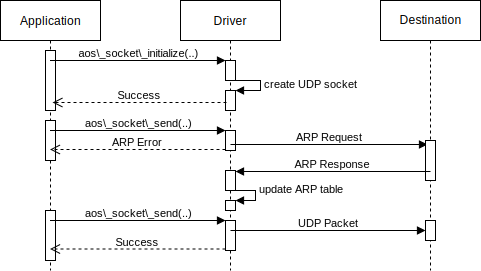
\includegraphics{networking/img/Sequence_Send.png}
    }
    \caption{Creating a Socket and Sending Data to a Remote Destination}
    \label{fig:enet_send}
    
\end{figure}

Receiving data over UDP is quite similar. After initiating a socket for a local port, an application can try to receive data over it. The driver will then check if there are any packets in that port's receive buffer. If there are, the driver will return the oldest one, and if the receive buffer is empty, the driver will report an according error:
\begin{mdframed}[style=myframe]
\begin{minted}[xleftmargin=\parindent,linenos,breaklines]{C}
struct *udp_msg = malloc(sizeof(struct udp_msg) + 2048);
errval_t err = aos_socket_receive(&sock, msg);
if (!err_is_fail(err)) {
    printf("received: \%s\n", msg->data);
}
\end{minted}
\end{mdframed}

Figure \ref{fig:enet_recv} shows an application trying to receive data over an already established socket. The first attempt fails as there is no data in its receive buffer. But afterwards, the driver receives data from a remote source which it then adds to the socket's receive buffer. Finally, the application's second attempt at receiving data succeeds, as now there is a packet in its receive buffer.

\begin{figure}[H]
\centering
    %\scalebox{0.9} {
    \resizebox{\textwidth}{!} {
        \includesvg{networking/img/Sequence_Receive.svg}
        %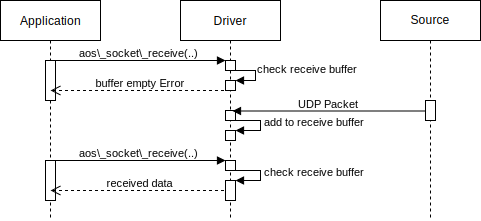
\includegraphics{networking/img/Sequence_Receive.png}
    }
    \caption{Receiving Data from a Remote Source}
    \label{fig:enet_recv}
\end{figure}

Similar to its UDP sockets, the library also provides an interface for sending ICMP echo requests and handling echo replies. For each target IP address, the driver keeps track of the last sent request's seqno as well as the highest acknowledged seqno. When an application tries to send the next echo request, the driver either retransmits a not yet acknowledged request, or if all requests have been acknowledged, sends a new request. Additionally, an application can request the highest seqno that has been acknowledged so far. The methods surrounding ICMP sockets are analog to the ones surrouning UDP sockets. For a simple example of them being used, see \C{usr/ping/main.c}.

\hindsight{
If the explanation of ICMP sockets seems rushed, then that is because their implementation was a bit rushed too. In hindsight, it would have been better to already consider requirements for ICMP messages when first writing the \C{udp\_service} library. Unfortunately, I first designed a library catered only towards sending and receiving UDP packets and only after it was working did I add ICMP ports and a \C{ping} application.
}

Perhaps the simplest method in this library is \C{aos\_arp\_table\_get}. It simply writes the device's current ARP table to a target buffer. Due to its simplicity, the function does not require any kind of socket to be initialized. Instead, it creates a new channel to the ethernet driver, requests the current ARP table, copies it to the target address and frees all data it allocated:
\begin{mdframed}[style=myframe]
\begin{minted}[xleftmargin=\parindent,linenos,breaklines]{C}
char *msg = malloc(2048);
aos_arp_table_get(msg);
print(msg);
\end{minted}
\end{mdframed}

\comment{
While trying to verify my correct implementation of the various protocols and algorithms, I encountered several peculiar interactions with my laptop. For instance, any UDP checksum I computed was flagged as faulty by Wireshark and ultimately never made it to its destination. However, Wireshark also flagged any outgoint UDP traffic from my laptop as faulty too. What solved this issue was to simply set the checksum to 0.

Another, more confusing issue I encountered was that any application (\emph{netcat, python,\dots}) running on my laptop was unable to receive UDP data from the Toradex board, unless Wireshark was running. I was unable to find the cause of this issue, but I found it interesting nonetheless.
}


\subsection{Networking Utilities}
Using the \C{udp\_service} library described above, I implemented a small selection of networking related programs. All of them can be started from \C{josh}.

\subsubsection{The arp Application}
The \C{arp} application (\emph{or \emph{"arplication"} for short}) simply requests the current ARP table from the driver, prints it and then terminates. It takes no arguments, but it does its best to provide aesthetically pleasing output. Listing \ref{enet:pingdemo} illustrates a possible output of this application.

\subsubsection{The ping Application}
The application \C{ping} creates an ICMP socket and uses it to send ICMP echo requests to a target IP address. It continuously updates the user on any received acknowledgements and keeps transmitting until the requested number of packets have been acknowledged. Its first argument is the target IP addres, and its second argument is the number of packets to have acknowledged. While it does not provide advanced features like packet multicasting, packet scheduling or time measurements, it still has its use cases. For instance, it can be used to indirectly trigger ARP requests when used on a new destination. Listing \ref{enet:pingdemo} shows how an initially empty ARP table can be extended after pinging a new destination.

\begin{code}
\begin{mdframed}[style=shell]
\josh{arp}\\
=========== ARP Table ===========\\
=================================\\
\\
\josh{ping 169.254.6.85 3}\\
pinging 169.254.6.85, 3 times\\
packet 1 was acked\\
packet 2 was acked\\
packet 3 was acked\\
\\
\josh{arp}\\
=========== ARP Table ===========\\
169.254.6.85\ \ \ \ \ \ 3e:1f:f:7:3:1\\
=================================
\end{mdframed}
\caption{Demonstration of \C{ping} causing ARP lookups}
\end{code}
\label{enet:pingdemo}

\subsubsection{The echoserver}
Finally, for an application built on UDP sockets, we have the \C{echoserver}. It takes a single argument, namely the port on which the server is to listen for incoming data. It then keeps receiving data on that port, and responds to any incoming data by sending an exact duplication back to its origin. Any device connected to the board can then send UDP packets to it and receive the exact same payload as reply. Listing \ref{enet:echodemo} show a remote device connecting to and using the echoserver with netcat.

\begin{code}
\begin{mdframed}[style=shell]
\bash{nc -u 10.0.2.1 4999}\\
Grow up Mr. Bond\\
Grow up Mr. Bond\\
Shaken, not stirred\\
Shaken, not stirred
\end{mdframed}
\caption{Demonstration of the Echo Server}
\end{code}
\label{enet:echodemo}

An earlier version of the echoserver was built directly inside the ethernet driver. With it, the driver had a separate handler it used for UDP packets arriving on port 2521. This handler created a reply with identical payload and sent it back to the source. While this version is not present in the driver's current form, it can be added back by adding the line \C{#define STATIC\_UDP\_ECHO 1} to the file \C{usr/drivers/enet/enet\_handler.c}.

Due to its simplicity, the echo server will be the main component of all performance measurements carried out below.

\subsection{The M-Shell}
The last application built using my \C{udp\_service} library is \C{msh} -- the M-shell. It allows users to connect to josh, our operating system's shell, over the internet. Since josh got their name from James Bond, and my remote shell essentially serves as a way to issue orders to josh, it seemed fitting to name my shell after "M" -- James Bond's boss. Luckily, \C{msh} has much more direct control over josh than M over Bond, so users will not have to worry about josh violating international law or going rogue on a quest for revenge.

Starting \C{msh} is very similar to starting an echo server: it only takes the port to listen on as argument. Once started, it first spawns a new \C{josh} process. But unlike the regular \C{josh} process spawned automatically at startup, this one does not read from and write to the serial port. Instead, \C{msh} has two data channels with this new process, one for \C{stdin} and one for \C{stdout}. Now \C{msh} can send any input for \C{josh} through one data channel and receive the output from the other one.

After spawning its own \C{josh} instance, \C{msh} then listens for incoming data on the specified port. It responds to the first message with a welcome message, but afterwards it simply forwards any UDP data to \C{josh} and sends any output it receives from \C{josh} back to the remote user.

Figure \ref{fig:msh_design} shows how this design works when a user attempts to evaluate the command \C{"echo a"} over my remote shell. It also illustrates an unexpected peculiarity: \C{josh} immediately writes every input it receives back to its \C{stdout} in order to give the user an immediate response to what they are typing. My remote shell will therefore also immediately echo every command it receives, and only then will it send back the output the command. To avoid confusion, the user is advised to disable their own terminal emulator from echoing back any key stroke. For a more responsive shell it is also advised to configure the terminal emulator to send each character immediately instead of sending data by lines. See listing \ref{enet:msh_demo} for an example of a user setting these recommended options and connecting to and using \C{msh}.

\begin{figure}[H]
\centering
    %\scalebox{0.9} {
    \resizebox{\textwidth}{!} {
        \includesvg{networking/img/msh_design.svg}
        %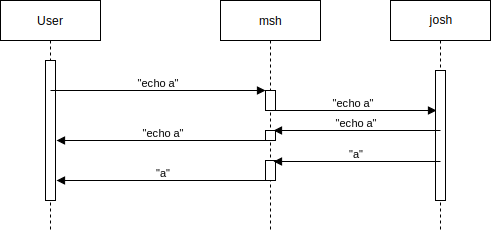
\includegraphics{networking/img/msh_design.png}
    }
    \caption{Receiving Data from a Remote Source}
    \label{fig:msh_design}
    
\end{figure}

\begin{code}
\begin{mdframed}[style=shell]
\bash{stty -icanon -echo \&\& nc -u 10.0.2.1 5000}\\
\\
\ m\ \ \ \ m\ \ mmmm\ \ m\ \ \ \ m\\
\ \#\#\ \ \#\# \#"\ \ \ " \#\ \ \ \ \#\\
\ \# \#\# \# "\#mmm\ \ \#mmmm\#\\
\ \# "" \#\ \ \ \ \ "\# \#\ \ \ \ \#\\
\ \#\ \ \ \ \# "mmm\#" \#\ \ \ \ \#\\
\\
\josh{@2 arp}\\
=========== ARP Table ===========\\
169.254.6.85\ \ \ \ \ \ 3e:1f:f:7:3:1\\
=================================\\
\end{mdframed}
\caption{Setting Recommended Settings and Using netcat to Connect to \C{msh}}
\end{code}
\label{enet:msh_demo}

An especially cool thing about this remote shell is that with the above command, it really does provide the exact same experience as using \C{josh} directly on the board itself. Not only do the color escape codes work seamlessly, but also the arrow keys, backspace and CTRL+L to clear all work as well.

\subsection{Performance Measurements}
Since UMP messages offer the most flexibility among the implemented features, I carried out all of my performance measurements by having the Toradex board run one or many UMP echo servers. On a connected computer I then ran python scripts to send messages of various length to the board and measure how long it takes for the echo reply to be received.

\subsubsection{Single Server}
For the first benchmark I had one echoserver running on the Toradex board. On my laptop I then ran a python script which sent messages of increasing payload size. For every message it sent, it measured how long it took for the corresponding answer to arrive. Each message size was sent a total of $4'096$ times and the response time was averaged over all iterations. Lastly, for the messages themselves I used part of the lyrics to \emph{Fool for Love} by \emph{Lord Huron}. While that last detail is not directly relevant to the results themselves, it is a great song and I will use every chance to mention it. 

I ran this first experiment a total of three times. One time the echo server was running on core 0, once it was running on core 1 and once it was running inside the ethernet driver itself (\emph{see Figure \ref{fig:single_echo})}. Unsurprisingly, the server inside the driver had by far the lowest latency. Since the incoming data never had to make the detour to a separate process before being sent back, the board was able to respond the quickest out of all tested configurations. Furthermore, running the echo server outside the driver but on the same core results in the highest latency, while running it on a separate core is only slightly worse than running it inside the driver. These results are not surprising, as processes sharing the same core can often interfere with each other, leading to performance losses and thus higher latency.
%Additionally, our measurements from section \ref{mp:perf_subs} also showed better performance for UMP channels than for LMP, 

\begin{figure}[H]
\centering
    \resizebox{\textwidth}{!} {
        \includesvg{networking/img/single_echo.svg}
    }
    \caption{Benchmarking Latency for a Single Echo Server Instance}
    \label{fig:single_echo}
\end{figure}

\subsubsection{Multiple Servers}
To benchmark my network stack's latency under a higher load, I had multiple echo servers running on different ports. Based on my previous results I ran all of them on cores 1-3. For each running server I had one agent on my laptop repeating the previous test. This experiment was done with up to 10 echo servers, each communicating with a separate measuring agent. Figure \ref{fig:para_echo} shows the average latency for varying numbers of servers and different message sizes.

\begin{figure}[H]
\centering
    \resizebox{\textwidth}{!} {
        \includesvg{networking/img/para_echo.svg}
    }
    \caption{Latency for Multiple Single Echo Server Instances}
    \label{fig:para_echo}
\end{figure}

Unsurprisingly, the latency increases significantly with more servers running in parallel. Especially for short messages, a low number of threads produces much better performance, as even very short waiting periods for any of the servers have an immediately visible effect on the overall latency. For larger message sizes on the other hand, even messages that get handled without ever waiting for the driver take quite a while to travel to the echo server, back to the driver and then back to the remote device. As a result, a higher number of running servers is much less noticeable. In fact, for very long messages, the latency was virtually identical for all measurements taken with 1-3 running servers.

\subsubsection{Bandwidth Measurements}
While low latency certainly is desirable, it is useless without an acceptable bandwidth to go along with. My last measurements were therefore trying to find my network stack's maximum bandwidth. For this I had one thread on my laptop send packets of size 128 to the Toradex board at a constant bandwidth for 5 minutes, while another thread was receiving and counting all the data coming in response. Meanwhile, there was a single echo server running on the Toradex board's core 1. This was then repeated for several different bandwidths, producing the red results shown in Figure \ref{fig:bw_echo}.

\begin{figure}[H]
\centering
    \resizebox{\textwidth}{!} {
        \includesvg{networking/img/bw_udp.svg}
    }
    \caption{Bandwidth of a Single Echo Server Instance}
    \label{fig:bw_echo}
\end{figure}

As can be seen, my network stack can easily achieve bandwidths of up to $190 \frac{MB}{s}$, as it was comfortably able to keep up with the load up to that point. For loads beyond that, the initial version of my stack was no longer able to keep up, and for roughly $1.2 \frac{GB}{s}$ it stopped working entirely, because the nameservice shut it down. Since my ethernet driver's initial version always checked for new packets before it checked for incoming RPCs, a too high network load lead to the ethernet driver being unable to respond to any other processes on the device itself. In response, the nameserver assumed the driver had stopped working and removed it. Luckily, this issue was easy to ammend simply by reprogramming the ethernet driver to first dispatch any RPCs before checking for incoming packets.

Indeed, implementing this small change inside the ethernet driver produces the much better blue results. The driver is now able to reach almost twice as high bandwidths, and even when the echo server is no longer able to keep up with the offered load, the driver does not stop working entirely. Instead it still achieves bandwidths higher than the previous driver version did most of the time.

% stty -icanon -echo && nc -u 10.0.2.1 1525
\section{The File-system}\label{filesystem}

A working operating system cannot only function from ram. It needs a storage medium and with that there comes the need for a file-system. 

As my personal project, I did my best to use the functionality of the already implemented sdhc reader/writer and implemented parts of the fat32 file-system so that access to the inserted SDHC card is made possible. 

\subsection{Core Functionality \& Overview}
The terminology user is in the following chapter used equally to a process. 

The main purpose of the file-system and driver blackbox (for now at least) is to provide processes the access to a storage medium, the sdcard. With the access there comes the need for \emph{read}, \emph{write}, \emph{create} and \emph{delete} files and directories as well as retrieving the attributes they come with. 

The user can use this functionality by either including \C{<aos/fs\_service.h>} and use the commands 

\begin{mdframed}[style=myframe]
\begin{minted}[xleftmargin=\parindent,linenos,breaklines]{C}
void read_file(char *path, size_t size, char *ret);

void write_file(char *path, char *data);

void delete_file(char *path);

void read_dir(char *path, char **ret);

void create_dir(char *path);

void delete_dir(char *path);
\label{code:fsserv}
\end{minted}
\end{mdframed}

or just by using the following commands in josh (the shell). 

\begin{mdframed}[style=shell]
\josh{cat "\emph{path}"}

\josh{wtf "\emph{path}" "\emph{text}"}

\josh{rm "\emph{path}"}

\josh{mkdir "\emph{path}"}

\josh{ls "\emph{path}"}

\josh{rmdir "\emph{path}"}
\end{mdframed}

Please note that every path has to start with \C{"/sdcard"} as this is the requested root folder.

Now, this is a good place to talk about what my file-system is capable of. Sadly, it cannot do all the things I wished it could. I had to make some assumptions which I am going to talk about later on. The following list contains the functionalities I implemented successfully:

\begin{itemize}
\item Mounting the SDHC card at $/sdhc$
\item FAT32 entries are only of type \emph{short entry}
\item Creating files on the SDHC card
\item Reading files on the SDHC card
\item Writing at the end of files on the SDHC card
\item Truncate files on the SDHC card to a defined size
\item Creating folders on the SDHC card
\item Deleting folders on the SDHC card
\item Retrieving information on the folder/file on the SDHC card
\item No access conflicts with multiple processes on different cores
\end{itemize}

\subsection{Implementation}
The already implemented ram-file-system was a guideline for me and helped me understand how the connection between the c library call and the function call accessing the storage medium works. I am positive that I did not understand it completely. It was though a good example how important documentation is. 
At some later point in time it seemed a good idea to not only use the ram-file-system as a guideline but to follow the structure as rigid as possible. The reason for that was that I lost a lot of time in trying to understand the functionality/complexity of those calls and coming up with my own without any documentations on the inputs or output and I preferred a working system instead of some idea of a system.

To understand the fat32 format the fact-sheet provided was enough. Fascinating to see was that some things essential to me were missing when formatting the SDHC card on Linux. 

Here a small illustration how the pipeline works and therefore which parts the user needs to know about:

\begin{figure}[h]
    \centering
    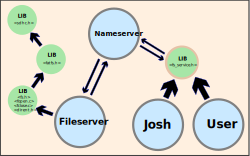
\includegraphics[width=0.9\textwidth]{./filesystem/data/fileaccess.png}
    \caption{Illustration of the file-system pipeline}
    \label{fig:ns_rtt}
\end{figure}

\subsubsection{FATFS library}
I implemented the main functionality/functions as a libraries of the file-system. They provide the connection between user and storage device. The communication (data transfer) between the SDHC driver and a server is done over the first slot in the ARG-CNODE. 

Important to note is the following terminology. The sdcard formatted as FAT32 consists in my case of clusters, which consists of sectors, which consists of bytes.

\subsubsection{Initializing/mounting}
The initialization consists of mounting the SDHC card to the folder "/sdcard" and connecting the fatfs functions to the c library function (fopen, fwrite, opendir, etc.). Mounting includes the creation of the \C{struct fatfs\_mount} which is crucial across all file accesses. 
The struct contains global information like the connection point to the sdcard (\C{struct sdhc\_s}), the directory entry for the root folder and the state of the FAT32 file-system (\C{struct fat32\_fs}). 

The state of the FAT32 file-system contains all info's about the FAT32 file-system inserted into the SDHC slot. Important to mention is the buffer page. It is an allocated frame mapped in the virtual address space, where the exchange between user and memory happens, the sdhc driver the connects the memory to the sdcard. The allocated frame is in my case not cached and therefore cache invalidation should theoretically not be necessary. 

With all these info's, manipulating bytes from/on the sdcard is possible.

\subsubsection{FAT Table-walk}
The FAT table-walk needs three operation types: 
\begin{itemize}
\item Retrieve the index of a free cluster
\item Get the next connecting cluster
\item Manipulate an entry
\end{itemize}

Thus only three functions are needed. In regard to retrieving a free cluster, all bytes in that cluster are zero'ed. It makes debugging as well as creating files in a cluster belonging to a folder less error-prone if your code is not perfect. As mine is not perfect, I encountered some conflicts with Linux formatting the sdcard, especially the root-folder. But more in the "Compromises / Encountered obstacles" section \ref{subsec:comp}.

\subsubsection{Directory-entries (dirent)}
A file or folder is always 32 Bytes on the FAT32 file-system and is called a directory-entry or dirent. Of course only under the assumption that there are only short FAT32 entries. On opening such an entry, a handle (\C{struct fatfs_handle}) is created containing the status and dirent info (\C{struct fatfs_dirent}) of the entry.

\begin{mdframed}[style=myframe]
\begin{minted}[xleftmargin=\parindent,linenos,breaklines]{C}
struct fatfs_handle
{
    struct fs_handle common;        ///< fatfs_mount pointer
    char *path;                     ///< string containing the path
    bool isdir;                     ///< offset in bytes
    struct fatfs_dirent *dirent;    ///< flag indication this is a dir

    off_t file_pos;                 ///< file content offset in bytes
    off_t dir_pos;                  ///< folder position offset in bytes
};

struct fatfs_dirent
{
    char *name;                     ///< name of the file or directory
    size_t size;                    ///< the size of the direntry in bytes or files
    struct fatfs_dirent *parent;    ///< parent directory

    uint32_t cluster;               ///< cluster number
    uint32_t sector;                ///< sector number
    uint32_t sector_offset;         ///< offset of sector to entry in bytes
    uint32_t content_cluster;       ///< cluster containing data or folder entries

    bool is_dir;                    ///< flag indication this is a dir
};
\end{minted}
\end{mdframed}

The name of an entry has an explicit length and way to be written into the FAT32 structure, therefore a translation between those two styles had to be done before comparing those two (useful when trying to find an entry).

\paragraph{File manipulation}
Regarding the fields contained in the handle struct and the ease of access to the entry on the sdcard, the functions \emph{open}, \emph{read}, \emph{write}, \emph{create}, \emph{truncate}, \emph{tell}, \emph{seek}, \emph{close}, \emph{stat} and \emph{remove} for files the implementation was not that simple as the operation the functions should perform was not clear. They were not intended to be called directly by the user but to be used by the standard c library functions. Those seemed to have an own agenda for what they use those functions and in the end it is still a mystery to me what some of those want from me.

In the case of writing, I made the assumption to only be able to write at the end of a file and therefore enlarging it. I did that regarding the time I had to understand the "blackbox" between the c library call and my function calls and the remaining time to come up with a working implementation.

Concerning the creation of a file: An empty file has no cluster containing the content. It is created as soon as the first write is attempted. 

Now comes the part where I thought I made a breakthrough understanding the c library calls. On reading, the function actually does not have to read the full required length. A small fraction suffices. The function calling my implemented read function is apparently a loop which calls my read function as long, as something readable is returned and concatenates the results. Therefore I was able to break down the implementation of the read function greatly into only reading chunks of a the size of a sector or until the sector-end.  

\paragraph{Folder manipulation}
Again, regarding the fields contained in the handle struct and the ease of access to the entry on the sdcard, the functions \emph{open}, \emph{create}, \emph{read\_next}, \emph{close} and \emph{remove} were equally problematic as those for files. 

On creating folders two "link-folders", namely "." and "..", are created. Those folders are only links and therefore don't have to be removed explicitly before removing a folder. The folder must though only contain those two link folders upon removal. 

\subsection{File-system-server or "Solving concurrent access"}
Now that the library was implemented, a server function which calls those functions seemed reasonably intelligent. This because then I had the problem of interfering concurrent accesses solved and it was not that complicated to implement. This compromise with on the other hand a loss in speed made the decision. 

The file-system-server is connected to the name-server and awaits incoming file-access-requests. Including a handler function, which handle incoming file-access-requests, the server also initializes and mounts the file-system. Important to note is that the init-process has to wait until the server registered the handler on the name-server. Otherwise file-access-requests grant an error. 
I went for the registration of a handler function on the name-server over an RPC-call because the connection between caller and callee is direct and the interface matches the requirements of the file-system-server.

\subsection{File-system service}
The file-system service implemented as a library in \C{<aos/fs\_service.h>} connects the user (over the name-server) with the file-system-server. These \ref{code:fsserv} functions allow him to access the file-system on the sdcard. 

Interesting to point out is that the message sent over the name-server has always the same structure. The type field sent along the message is the identifier what the call actually should execute on the other side and also defines the return value.  

\subsection{Compromises / Encountered obstacles}
\label{subsec:comp}

\subsubsection{SDHC reads and the Cache}
As mentioned before, the allocated frame, which connects the user to the ram is not cached. Unfortunately there were some delays between reading/writing and accessing the the read bytes from the sdcard on the memory. I did not find out why it had delays. Invalidating the cache before a read with a memory barrier or flushing the cash before a write with a memory barrier had no effect. 
I encountered this problem as I removed the \C{debug\_printf} statements and imitated those delays with an volatile for-loop. This fix is ugly but it does the trick (for now).

\C{for (volatile int t = 0; t < 1000000; t++);}

Analysing this bug was a dead end. The label \C{NOCACHE} was successfully loaded into the pagetable and debugging the sdhc driver was not successful as the debug messages showed no sign of failure.

\subsubsection{Formatting on Linux}
Interesting to see was that formatting on Linux did not set the cluster containing the entries in the root folder to zero or delete the files in it. This was quite the hustle, as I thought I did something wrong but it seemed the attribute was set to zero. It is still quite a mystery to me, what Linux understands under formatting. The specs sheet of FAT32 clearly commands you to set all entries in a newly assigned cluster for a folder to zero.

\subsection{Measurements/Performance}
I did some measurements on the function call writing and reading to the sdcard (\C{<sdhc.h>}). For stability reasons I performed the following measurements 100 times.
\begin{itemize}
\item Sequential sdhc\_read: 475ms
\item Sequential sdhc\_write: 475 ms
\item Alternating sequential read/write's: 955 ms
\end{itemize}

This indicates, that on switching from read to write or vice versa, 5 ms are lost somewhere. 

Now comes the interesting part. I measured the fastest time for each file-system call (\C{fs\_service.h}). 
After 10 iterations it was clear, that the values are always the same.
Important to note is, that writes and reads with large content increase in time, every new sector. This makes sense as every new sector has to be loaded and written to the sdcard.

\begin{itemize}
\item Sequential write\_file (incl. creation): 924 ms
\item Sequential read\_file:  90 ms
\item Sequential remove\_file: 406 ms
\item Sequential create\_dir: 863 ms
\item Sequential read\_dir: 172 ms
\item Sequential remove\_dir: 341 ms
\end{itemize}

The quick-fix for the sdhc driver increases the time for every read/write from/to the sdcard by 20 ms. 

Now, the attentive reader may have noticed, that the "Sequential sdhc\_read" take way more time than the direct "Sequential read\_file". But it should not! The "Sequential sdhc\_read" is called in the "Sequential read\_file", so the later should take more or equal the amount to time of the first. The only way I can think of explaining this phenomenon is that the first measurement is called right after initializing the file-system and the second one is called from user space. Therefore some optimizations/caches probably happen between those two calls. 

\subsection{Improvements}
This is clearly not best solution for implementing a file-system. I would even go as far as it is not even a good one. Improvement can be done from the beginning. I will not go into functionalities which I did not implement. Concerning speed, the sdhc bug would give us some speedup. But it is not significant. More interesting I think is that most of the time is lost due to the read and writes to and from the FAT table and FOLDER ENTRIES to the same sectors. Thus a cache or a bigger buffer (currently only one sector) would in most cases result in a speedup. The principles of temporal locality and spacial locality can be applies to storage media (at least at some scale).

All in all this could bring some speedup but the worst case remains the same. 

Furthermore understanding the c lib function calls will help to further break down my implemented functions to a simpler constructs with possible speed gain. The other way is also possible, instead of breaking down the functions, implement an algorithm which solves the request directly. I am thinking of the \C{fatfs_read} function, where I only return chunks of the requested file. If I returned the full requested read size, then the usage of the buffer-page will be better.

Concerning work allocation, right now there is only one process managing the whole file-system. I could imagine some speedup if there were multiple processes for managing the FAT, the DATA section or even each individual function calls. As interesting this sounds, the problems it comes with are another hurdle. With this idea, concurrency and race-conditions become a real problem and the concept has to stand before one can even attempt to program such a structure. 
\section{Acknowledgements}

We would like to thank Professor Dr. Roscoe and Dr. Cock for organizing the course. Furthermore, we appreciate all the TAs who helped fixing bugs during development and organizing the coffee and chat sessions in times of corona. Last, but most certainly never least, we would like to thank Lord Huron for making absolutely fantastic music.


\newpage
\section{Appendix}\label{appendix}
\subsection{Notable Bugs We Encountered}
During the project, as our project grew bigger and more complex, we encountered many bugs, sometimes
really hard to find ones.

In this section we compiled some stories of the most infamous bugs we had to defeat on our journey through AOS.

\subsubsection{RPC calls non-reentrant bad?}
When we first created a process manager as a separate dispatcher that was supposed to keep track of every
running dispatcher, we encountered an RPC call that never returned.

In the init-dispatcher, whenever we spawned a new dispatcher, we notified the process manager via an RPC.
Said RPC however never returned.


The not-immediately obvious reason for this was that our \C{struct aos_rpc} framework is non-reentrant, i.e.
while we call from A to B via such a struct, we can't call back to A from the handler in B. This could actually be
implemented without too much hassle (probably), however we chose not to, but instead only ever use RPCs in one direction.

In this case, we were however accidentally doing exactly that, as the channel we used to send the
``new-process''-notification to the process manager was the same channel the process manager used to request
ram capabilities when in need.

Weirdly enough, we ensured carefully that we did not allocate any memory in the notification handler in the process manager.
Still, instead of an ACK-style response to the new-dispatcher-notification, we got a ram request.

A few days earlier, we implemented the lazy allocation for heap memory as well as for stack memory.
We grew fond of a lazily allocated stack and assumed it would be a good thing to have all stacks in the
system lazily allocated, including the main thread stack for every dispatcher. We even switched out the
main thread stack in the init dispatcher for a lazily allocated one.

In our specific case here however, it backfired rather badly. Although we tried not to allocate any memory while
in a rpc handler, we did not account for the possibility that at any moment when writing to the stack, we might
encounter a page fault and request a frame from init.
\begin{figure}[ht]
    \centering
    
        \scalebox{0.7}{
            \hspace{-0.40in}
            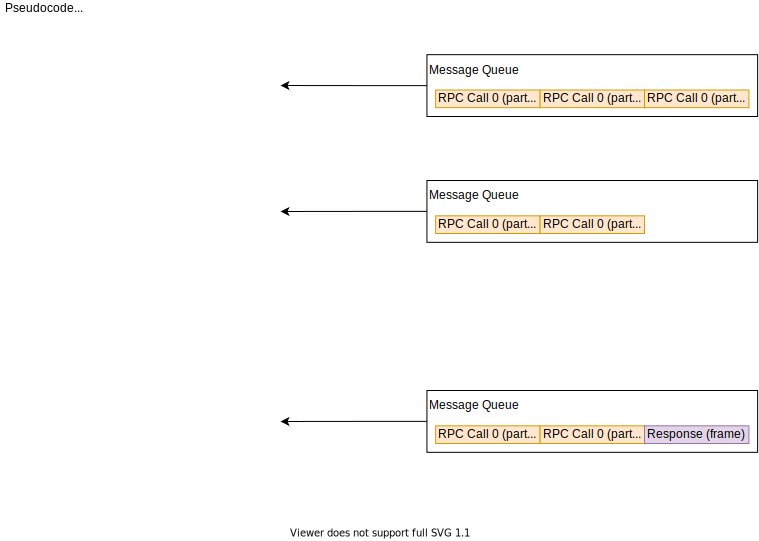
\includegraphics{./bugs/memoryreq.pdf}
        }
    % \vspace{-1in}
    % \caption{Example bug encountered during for our RPC implementation}
    % \label{fig:bug_mm_req}
    
\end{figure}




\end{document}
